% =======================================================================================================
% Capítulo 4 - Resultados e Discussão
% =======================================================================================================

Este capítulo apresenta os resultados na mesma ordem do Capítulo~\ref{chap:metodos}: o ensaio do extrator de \textit{hits} contra o sistema comercial (Seção~\ref{sec:res_extrator}), a classificação das condições da bomba a partir dos registros (Seção~\ref{sec:res_bomba}), a implementação embarcada da classificação (Seção~\ref{sec:res_embarcado}) e a validação externa na base CWRU (Seção~\ref{sec:res_cwru}). A Seção~\ref{sec:discussao_integrada} reúne os resultados para responder às questões que motivaram o trabalho.

% -------------------------------------------------------------------------------------------------------
\section{Extrator de \textit{hits}: ensaio simultâneo com o AMSY-6}
\label{sec:res_extrator}
% Gerado por ferramentas/importar_relatorios.py a partir de ARTIGO_V2-10.11.2026/6-Resultados_discussao2.tex.
% Revisado à mão na dissertação: edite este arquivo, não a fonte.
% =======================================================================================================

Esta seção apresenta os resultados dos ensaios descritos na Seção~\ref{sec:mm_delineamento}. Ela reúne os resultados preliminares obtidos até o momento e o plano de análise para as condições ainda não ensaiadas.

Nenhum resultado esperado é incorporado antecipadamente à redação. Em particular, não se pressupõe convergência para 100\% de detecção em amplitudes elevadas, superioridade de um dos sistemas próximo ao limiar, subestimação obrigatória das contagens ou adequação ao Projeto MOMEA. Essas hipóteses podem orientar a investigação, mas as conclusões decorrem dos dados, das incertezas e dos critérios de aceitação previamente definidos.

Os resultados apresentados são os da sessão simultânea R1 (15/10/2026: bursts senoidais de 10 ciclos a 50, 200 e 450\,kHz, \(\approx 95\,\mathrm{dB}_{\mathrm{AE}}\), pré-amplificadores de 34\,dB, blocos de 1 a 10\,000 \textit{bursts} em 30\,s). Eles são identificados como preliminares porque ainda faltam as repetições independentes da sessão, a referência elétrica medida no osciloscópio e a varredura de amplitude e SNR. Nas partes ainda sem dados, o texto descreve o plano de análise.

A apresentação distingue:
\begin{enumerate}
	\item Desempenho de detecção e de segmentação;
	
	\item Erro dos descritores em relação à referência elétrica independente;
	
	\item Concordância entre o sistema proposto e o AMSY-6;
	
	\item Influência do plano de injeção e das configurações instrumentais; e
	
	\item Desempenho computacional, integridade da comunicação e redução do volume de dados.
\end{enumerate}

% -------------------------------------------------------------------------------------------------------
\subsection{Integridade dos dados e população analisada}
\label{v2:subsec:integridade_resultados}

Antes de qualquer comparação paramétrica, é apresentada a rastreabilidade dos estímulos e registros. Para o sistema proposto, os contadores documentam, quando disponíveis:
\begin{equation}
	N_{\mathrm{ger}} \longrightarrow N_{\mathrm{FSM}} \longrightarrow N_{\mathrm{DMA}} \longrightarrow N_{\mathrm{tx}} \longrightarrow N_{\mathrm{rx}}
	\label{v2:eq:fluxo_contadores_resultados}
\end{equation}

\noindent
em que \(N_{\mathrm{ger}}\) é o número de estímulos aplicados, \(N_{\mathrm{FSM}}\) é o número de registros consolidados pela lógica, \(N_{\mathrm{DMA}}\) é o número entregue ao caminho de memória, \(N_{\mathrm{tx}}\) é o número transmitido e \(N_{\mathrm{rx}}\) é o número recebido e validado pelo computador hospedeiro.

As diferenças entre contadores consecutivos são apresentadas separadamente. A condição \(N_{\mathrm{rx}}<N_{\mathrm{FSM}}\), por exemplo, não demonstra falha de detecção; ela indica perda posterior à máquina de estados. Para o AMSY-6, são preservados e reportados os indicadores de saturação, \textit{timeout}, enchimento de \textit{buffer}, modo de longa duração e demais estados relevantes disponibilizados pelo sistema \cite{vallen2022}. Para cada condição experimental, são informados:

\begin{itemize}
	\item Número de estímulos programados e confirmados pela forma de onda de referência;
	
	\item Número de \textit{hits} produzidos por cada sistema;
	
	\item Número de estímulos sem registro associado;
	
	\item Número de associações unívocas, fragmentações e fusões;
	
	\item Número de falsos \textit{hits} nos intervalos contendo apenas ruído;
	
	\item Número de registros saturados, encerrados por \textit{timeout}, com transbordo ou com outro indicador de exceção;
	
	\item Número de perdas, duplicações e registros fora de ordem em cada camada observável; e
	
	\item Número e motivo das exclusões realizadas antes de cada análise.
\end{itemize}

\textbf{Resultados preliminares (R1).} A Tabela~\ref{v2:tab:fluxo_r1} resume a seleção dos registros na sessão R1, com as três frequências somadas. Na versão ensaiada, \(N_{\mathrm{FSM}}\) corresponde ao \texttt{HITCNT}, \(N_{\mathrm{DMA}}\) e \(N_{\mathrm{tx}}\) aos contadores do \textit{firmware} e \(N_{\mathrm{rx}}\) ao total gravado; não houve diferença entre \(N_{\mathrm{FSM}}\) e \(N_{\mathrm{rx}}\).

\begin{table}[htbp]
	\centering
	\footnotesize
		\caption{Seleção dos estímulos e registros na sessão R1 (15/10/2026), três frequências somadas (preliminar).}
	\label{v2:tab:fluxo_r1}
	\begin{tabular}{|p{0.30\textwidth}|p{0.30\textwidth}|p{0.30\textwidth}|}
		\hline
		\textbf{Etapa} & \textbf{Sistema proposto} & \textbf{AMSY-6} \\
		\hline
		Estímulos programados & \multicolumn{2}{c|}{\(3 \times 16\,101 = 48\,303\) \textit{bursts}} \\
		\hline
		Registros recebidos & 48\,282 & 47\,009 \\
		\hline
		Excluídos fora dos blocos & 2 (desligamento das saídas do gerador no fim das capturas de 200 e 450\,kHz) & 3 (transitório de configuração do gerador no início de cada captura) \\
		\hline
		Registros de \textit{bursts} & 48\,280 & 47\,006 \\
		\hline
		Estímulos sem registro próprio & 23, todos explicados no detector: 20 absorvidos no rearme (\textit{hits} com ROVL) e 3 em 2 \textit{hits} fundidos & 1\,297; 1\,086 \textit{hits} com indicador R \\
		\hline
		Exclusões por SAT ou MAXDUR & 0 & --- \\
		\hline
		Perdas na comunicação & 0/48\,280 & --- \\
		\hline
	\end{tabular}
\end{table}


As regras de exclusão são definidas antes da inspeção dos resultados e aplicadas de maneira simétrica. Registros saturados ou fragmentados não são simplesmente descartados: sua frequência é um resultado do experimento. Eles podem ser excluídos de uma análise específica de linearidade ou concordância, desde que permaneçam contabilizados e sejam apresentados em estrato próprio. Regra proposta, a fixar antes da análise final: registros com SAT, MAXDUR ou acumulador saturado entram nas contagens de detecção e formam estrato próprio; ficam fora das análises de linearidade e de concordância dos descritores; e o número de cada caso é reportado. \textit{Hits} fundidos (contagens múltiplas do esperado) entram na análise de detecção como fusão. Nos ensaios até 15/10/2026, não ocorreu nenhum \textit{hit} com SAT ou MAXDUR.

% -------------------------------------------------------------------------------------------------------
\subsection{Desempenho de detecção e segmentação}
\label{v2:subsec:concordancia_deteccao_resultados}

A análise de detecção segue a regra de associação da Subseção~\ref{v2:subsec:metricas_comparacao}. Para cada sistema e condição, são apresentadas:
\begin{itemize}
	\item Proporção de estímulos com ao menos um \textit{hit} associado;
	
	\item Proporção de associações unívocas \(1{:}1\);
	
	\item Proporções de ausência de detecção, fragmentação e fusão;
	
	\item Taxa de falsos \textit{hits} por unidade de tempo de fundo; e
	
	\item Intervalos de confiança compatíveis com o delineamento em blocos.
\end{itemize}

Para expressar a amplitude em relação ao limiar em uma base comum, define-se:
\begin{equation}
	\rho_i = \frac{V_{\mathrm{pico,ref},i}}{V_{\mathrm{th,ref}}}, \qquad A_{\mathrm{exc},i} = 20\log_{10}\left(\rho_i\right)
	\label{v2:eq:amplitude_relativa_limiar_resultados}
\end{equation}

\noindent
em que \(V_{\mathrm{pico,ref},i}\) é a amplitude do estímulo medida no plano de referência e \(V_{\mathrm{th,ref}}\) é o limiar referido ao mesmo plano. Essa normalização é válida somente quando as conversões de ganho e limiar estão calibradas e quando a grandeza utilizada pelo comparador é compatível. Se os sistemas operarem sobre sinais de decisão distintos, os valores em volts e as configurações originais também são apresentados.

A probabilidade de detecção é representada em função de \(A_{\mathrm{exc}}\), ou da SNR, separadamente para frequências, durações e demais fatores capazes de alterar a resposta. A agregação de condições heterogêneas em uma única curva pode produzir uma transição artificialmente larga ou deslocada.

Quando a faixa de amplitudes contiver observações abaixo e acima da região de transição e o ajuste for adequado, pode-se utilizar um modelo binomial. Em sua forma mais simples, para o sistema \(j\),
\begin{equation}
	\operatorname{logit} \left[p_j\left(A_{\mathrm{exc}}\right) \right] = \beta_{0,j} + \beta_{1,j}A_{\mathrm{exc}}	\label{v2:eq:modelo_deteccao_logistico}
\end{equation}

\noindent
com:
\begin{equation}
	\operatorname{logit}(p) = \ln \left(\frac{p}{1-p}\right)
\end{equation}

Se houver agrupamento por aquisição ou bloco, emprega-se um modelo binomial de efeitos mistos ou outra abordagem que preserve essa dependência. Frequência, SNR, duração e sistema podem ser incluídos como fatores, com interações justificadas pelo delineamento. 

A amplitude relativa associada a uma probabilidade \(q\) é estimada por:
\begin{equation}
	A_{q,j} = \frac{\operatorname{logit}(q)-\widehat{\beta}_{0,j}}{\widehat{\beta}_{1,j}}
	\label{v2:eq:amplitude_probabilidade_deteccao}
\end{equation}

Podem ser reportados \(A_{50}\) e \(A_{90}\), acompanhados de intervalos de confiança. Esses valores não são extrapolados quando a matriz não abrange a probabilidade correspondente, quando a curva não é aproximadamente monotônica ou quando há separação completa sem informação suficiente para estimar a transição.

A afirmação de que diferenças próximas ao limiar decorrem exclusivamente da diferença nominal entre 12 e 16 bits é insuficiente. A interpretação considera ruído referido à entrada, ENOB, faixa de entrada, ganho, resposta dos filtros, quantização do limiar e convenção do sinal de decisão.

\textbf{Resultados preliminares (R1).} A Tabela~\ref{v2:tab:deteccao_r1} resume a detecção por frequência e a Tabela~\ref{v2:tab:carga_r1}, por bloco de carga. Como a associação foi feita por bloco (sem \textit{timestamp}), \(N_{1:1}\) é estimado como os registros com 10 contagens e sem ROVL. O sistema proposto detectou de 99,94 a 99,96\,\% dos \textit{bursts} por frequência, e o AMSY-6, de 96,8 a 97,6\,\%. Não houve fragmentação: todos os \textit{hits} do sistema proposto têm 10 contagens ou múltiplos de 10. Houve 2 fusões no sistema proposto em 50\,kHz, cobrindo 3 \textit{bursts} extras. Nos blocos de 1, 100 e 1000 \textit{bursts} (intervalos \(\ge 30\,\mathrm{ms}\)), nenhum dos sistemas deixou de registrar estímulos; as diferenças concentram-se nos blocos de 5000 e 10\,000, em que o intervalo entre estímulos (6 e 3\,ms) se aproxima do tempo de ocupação do canal (duração + DDT + RAT \(\approx 2{,}3\)--\(2{,}4\,\mathrm{ms}\)).

\begin{table}[htbp]
	\centering
	\footnotesize
		\caption{Detecção por frequência na sessão R1 (16\,101 \textit{bursts} por frequência; preliminar).}
	\label{v2:tab:deteccao_r1}
	\begin{tabular}{|c|c|c|c|c|c|c|}
		\hline
		 & \multicolumn{4}{c|}{\textbf{Sistema proposto}} & \multicolumn{2}{c|}{\textbf{AMSY-6}} \\
		\cline{2-7}
		\textbf{Freq.} & \textbf{Registrados} & \textbf{Detecção} & \textbf{ROVL} & \textbf{Fundidos} & \textbf{Registrados} & \textbf{Detecção} \\
		\hline
		50\,kHz & 16\,094 & 99,96\,\% & 4 & 2 & 15\,580 & 96,8\,\% \\
		\hline
		200\,kHz & 16\,092 & 99,94\,\% & 9 & 0 & 15\,716 & 97,6\,\% \\
		\hline
		450\,kHz & 16\,094 & 99,96\,\% & 7 & 0 & 15\,710 & 97,6\,\% \\
		\hline
	\end{tabular}
\end{table}

\begin{table}[htbp]
	\centering
	\footnotesize
		\caption{Registros por bloco de carga na sessão R1 (diferença em relação ao número de \textit{bursts} entre parênteses; preliminar).}
	\label{v2:tab:carga_r1}
	\setlength{\tabcolsep}{3pt}
	\begin{tabular}{|p{0.13\textwidth}|c|c|c|c|c|c|}
		\hline
		\textbf{Bloco (30\,s)} & \textbf{50\,kHz P} & \textbf{50\,kHz A} & \textbf{200\,kHz P} & \textbf{200\,kHz A} & \textbf{450\,kHz P} & \textbf{450\,kHz A} \\
		\hline
		1, 100 e 1000 & sem perda & sem perda & sem perda & sem perda & sem perda & sem perda \\
		\hline
		5000 (6\,ms) & 5000 (0) & 4983 (\(-17\)) & 4997 (\(-3\)) & 4975 (\(-25\)) & 4999 (\(-1\)) & 4985 (\(-15\)) \\
		\hline
		10\,000 (3\,ms) & 9993 (\(-7\)) & 9496 (\(-504\)) & 9994 (\(-6\)) & 9640 (\(-360\)) & 9994 (\(-6\)) & 9624 (\(-376\)) \\
		\hline
		\multicolumn{7}{|l|}{P: sistema proposto; A: AMSY-6.} \\
		\hline
	\end{tabular}
\end{table}


% -------------------------------------------------------------------------------------------------------
\subsection{Concordância e diferenças paramétricas}
\label{v2:subsec:concordancia_parametrica_resultados}

A análise paramétrica principal utiliza estímulos com associação unívoca nos dois sistemas. Os casos de saturação, \textit{timeout}, fragmentação, fusão e transbordo são apresentados separadamente. Para cada descritor, apresentam-se:

\begin{itemize}
	\item Distribuição dos valores de referência e dos valores produzidos pelos dois sistemas;
	
	\item Gráfico do sistema proposto em função do AMSY-6, com linha de identidade e escalas iguais;
	
	\item Gráfico de Bland--Altman das diferenças em função da magnitude;
	
	\item Viés, desvio-padrão das diferenças, limites de concordância e intervalos de confiança; e
	
	\item Resultados estratificados pelos fatores para os quais houver evidência de alteração do viés ou da dispersão.
\end{itemize}

O procedimento original de Bland--Altman é descrito em \cite{bland1986}. Como existem repetições por condição e por bloco, os limites de concordância consideram medidas repetidas ou são estimados em estratos homogêneos. A extensão metodológica para medidas repetidas é apresentada em \cite{bland1999}. Os estratos são as condições experimentais (frequência \(\times\) bloco de carga \(\times\) plano de injeção), e os limites são calculados por condição, ou por modelo de medidas repetidas com a sessão como bloco, com intervalos de confiança, somente para os descritores classificados como equivalentes ou assemelhados no Quadro~\ref{v2:qua:configuracao_pareada_secao5}; para contagens, reporta-se a distribuição das discordâncias. A simples aplicação de \(\overline{d}\pm1{,}96s_d\) a todos os pulsos, ignorando o agrupamento, pode subestimar a incerteza. O coeficiente de correlação, quando apresentado, permanece suplementar e não pode fundamentar afirmações de concordância.

O Quadro~\ref{v2:qua:interpretacao_descritores_secao6} organiza as verificações necessárias. As possíveis origens listadas não constituem diagnósticos automáticos; uma divergência pode resultar de mais de um mecanismo. Segundo a especificação do fabricante, o processamento convencional dos \textit{hits} no AMSY-6 opera a \(10\,\mathrm{MHz}\) \cite{vallen2022}.

\begingroup
\renewcommand{\tablename}{Quadro}
\footnotesize
\renewcommand{\arraystretch}{1.22}
\begin{longtable}{|
		>{\raggedright\arraybackslash}p{2.5cm}|
		>{\raggedright\arraybackslash}p{4.0cm}|
		>{\raggedright\arraybackslash}p{4.1cm}|
		>{\raggedright\arraybackslash}p{3.6cm}|}
	\caption{Análises e cuidados de interpretação para os descritores.}
	\label{v2:qua:interpretacao_descritores_secao6}\\
	\hline
	\textbf{Descritor} & \textbf{Apresentação mínima} & \textbf{Fontes plausíveis de diferença} & \textbf{Verificação necessária} \\
	\hline
	\endfirsthead
	\multicolumn{4}{c}
	{\tablename\ \thetable{} -- continuação}\\
	\hline
	\textbf{Descritor} & \textbf{Apresentação mínima} & \textbf{Fontes plausíveis de diferença} & \textbf{Verificação necessária} \\
	\hline
	\endhead
	\hline
	\multicolumn{4}{r}{Continua na próxima página.}\\
	\endfoot
	\hline
	\endlastfoot
	Amplitude & Volts no plano comum, \(\mathrm{dB}_{\mathrm{AE}}\), erro perante a referência, dispersão, Bland--Altman e linearidade. & Ganho calibrado, resposta em frequência, carregamento, faixa de entrada, fase de amostragem, quantização, não linearidade e saturação. & Calibração da cadeia completa e ensaios em frequência e amplitude. \\
	\hline
	Tempo de subida & Erro em tempo e em unidades da grade de processamento; diferenças em função de frequência, amplitude e duração. & Limiar, resposta transitória e fase dos filtros, instante do pico, amostragem, interpolação e definição da primeira ocorrência do pico. & Comparar formas de onda de referência e respostas impulsivas ou de grupo das cadeias. \\
	\hline
	Duração & Diferença em tempo e amostras, distribuição discreta e estratificação por DDT. & Primeiro e último cruzamentos, sinal de decisão, limiar, filtragem, quantização temporal e convenção de encerramento. & Confirmar que a duração termina no último cruzamento e não na expiração do DDT. \\
	\hline
	Contagens & Diferença inteira, distribuição das discordâncias e análise por frequência, amplitude e SNR. & Filtragem, limiar, sinal com sinal ou módulo, grade de processamento, histerese, DDT, fase relativa e ruído. & Não atribuir a diferença diretamente a \(8\) contra \(40\,\mathrm{MS/s}\); comparar as grades efetivamente utilizadas na extração dos descritores. \\
	\hline
	Energia & \(\mathrm{V^2s}\), eu, razão ou diferença em escala logarítmica, erro perante a referência e indicação de saturação. & Fator de escala, janela integrada, ruído, filtros, truncamento, saturação, largura do acumulador e arredondamento. & Comparar \textit{True Energy} com a integral quadrática definida na Subseção~\ref{v2:subsec:energia_ea}; tratar \textit{Signal Strength} separadamente. \\
	\hline
	Tempo de chegada & Diferença temporal, deslocamento inicial e deriva ao longo de cada aquisição. & Bases de tempo, sincronização, atraso dos filtros, limiar e regra de interpolação. & Medir ou estimar deslocamento e deriva; não interpretar tempo absoluto sem sincronização. \\
\end{longtable}
\endgroup

Se a diferença for proporcional à magnitude, a análise em escala logarítmica é mais apropriada, desde que os valores sejam positivos. Nesse caso, são reportadas razões geométricas e limites multiplicativos, e não uma mistura entre diferenças em escala original e logarítmica.

% -------------------------------------------------------------------------------------------------------
\subsection{Erro em relação à referência elétrica independente}
\label{v2:subsec:exatidao_referencia_resultados}

Esta análise compara os dois instrumentos com os descritores obtidos da forma de onda elétrica medida independentemente, conforme a hierarquia da Subseção~\ref{v2:subsec:sistema_referencia_experimento}. A referência possui incerteza e depende do plano de medição, da banda e do processamento \textit{off-line}.

Os parâmetros nominais dos estímulos (Subseção~\ref{v2:subsec:sinais_teste}) fornecem diretamente pico e energia do sinal ideal, mas não fornecem automaticamente todos os descritores observados após filtros, ruído, amostragem, limiar e DDT. Tempo de chegada, tempo de subida, duração e contagens são calculados sobre a forma de onda de referência efetivamente medida, empregando as definições da Seção~\ref{sec:fund_hits}.

Para cada descritor e instrumento, são apresentados os erros definidos na Seção~\ref{sec:mm_delineamento}, acompanhados de viés, MAE, RMSE e intervalos de confiança. A incerteza-padrão combinada da diferença pode ser representada, em uma forma geral, por:

\begin{equation}
	u_{\mathrm{c}}^2\left(e_x\right) = u^2\left(x^{(j)}\right) + u^2\left(x_{\mathrm{ref}}\right) - 2\operatorname{cov} \left(	x^{(j)}, x_{\mathrm{ref}}\right)
	\label{v2:eq:incerteza_erro_referencia}
\end{equation}

\noindent
em que a covariância é mantida quando o descritor do instrumento e o de referência compartilham fatores de calibração ou dados. O orçamento de incerteza é compatível com o modelo definido conforme o JCGM~100 \cite{jcgm2008}.

Uma conclusão de equivalência é defensável somente se os intervalos obtidos forem confrontados com tolerâncias previamente estabelecidas. Ser mais próximo da referência do que o outro instrumento não demonstra, por si só, adequação à aplicação.

\textbf{Resultados preliminares (R1).} Ainda não há descritores de referência: falta capturar no osciloscópio a forma de onda efetivamente injetada. A comparação entre os instrumentos na sessão R1, com a amplitude do sistema proposto recalculada para o ganho de 34\,dB, está na Tabela~\ref{v2:tab:descritores_r1}, e os valores por bloco, na Tabela~\ref{v2:tab:valores_bloco_r1}. Nesse ensaio, o \textit{software} de aquisição do sistema proposto estava configurado com ganho de 35\,dB, de modo que o limiar efetivo foi de \(81\,\mathrm{dB}_{\mathrm{AE}}\).

\begin{table}[htbp]
	\centering
	\footnotesize
		\caption{Descritores na sessão R1: sistema proposto \(\times\) AMSY-6 (preliminar).}
	\label{v2:tab:descritores_r1}
	\begin{tabular}{|p{0.22\textwidth}|p{0.20\textwidth}|p{0.20\textwidth}|p{0.20\textwidth}|}
		\hline
		\textbf{Descritor} & \textbf{50\,kHz} & \textbf{200\,kHz} & \textbf{450\,kHz} \\
		\hline
		Amplitude (\(\mathrm{dB}_{\mathrm{AE}}\)) & 95,78 \(\times\) 95,30 (\(+0{,}47\)\,dB) & 95,79 \(\times\) 95,04 (\(+0{,}76\)\,dB) & 95,88 \(\times\) 95,29 (\(+0{,}59\)\,dB) \\
		\hline
		Desvio-padrão da amplitude & 0,06 \(\times\) 0,05\,dB & 0,05 \(\times\) 0,06\,dB & 0,04 \(\times\) 0,07\,dB \\
		\hline
		Duração (\(\mu\)s) & 188,8 \(\times\) 226,4 & 47,19 \(\times\) 51,48 & 20,97 \(\times\) 22,84 \\
		\hline
		Duração (períodos) & 9,44 \(\times\) 11,32 & 9,44 \(\times\) 10,30 & 9,44 \(\times\) 10,28 \\
		\hline
		Contagens & 10 \(\times\) 11 (12 em 1,6\,\%) & 10 \(\times\) 11 & 10 \(\times\) 11 \\
		\hline
		Energia (razão proposto/AMSY-6) & 1,28 & 1,36 & 1,44 \\
		\hline
		Energia / (\(A^2/2 \cdot\) duração) & 0,95 \(\times\) 0,69 & 0,97 \(\times\) 0,78 & 0,98 \(\times\) 0,71 \\
		\hline
		Tempo de subida (\(\mu\)s) & \(87 \pm 58\) \(\times\) \(37{,}0 \pm 4{,}7\) & \(27 \pm 15\) \(\times\) \(5{,}34 \pm 0{,}05\) & \(10{,}2 \pm 6{,}5\) \(\times\) \(1{,}45 \pm 0{,}05\) \\
		\hline
	\end{tabular}
\end{table}

A diferença de amplitude, de \(+0{,}47\) a \(+0{,}76\,\mathrm{dB}\), soma a assimetria do divisor e a diferença de ganho entre os pré-amplificadores (34,00 e 34,22\,dB) e só poderá ser separada com o Experimento A. A dispersão da amplitude é pequena e semelhante nos dois sistemas (0,04 a 0,07\,dB). A duração do sistema proposto corresponde a 9,44 períodos em todas as frequências, coerente com a convenção de término no último cruzamento; a do AMSY-6 é maior e varia com a frequência, assim como a contagem de 11 (e 12 em 1,6\,\% dos \textit{hits} em 50\,kHz), o que é compatível com a contagem da oscilação após o fim do \textit{burst}. A energia do sistema proposto é coerente com sua amplitude e duração (razão de 0,95 a 0,98 em relação a \(A^2/2 \cdot t_{\mathrm{dur}}\)); a do AMSY-6 fica 22 a 31\,\% abaixo do que sua própria amplitude e duração indicam. Por isso, duração e energia são tratadas como descritores assemelhados, e não como erros de detecção. O tempo de subida do sistema proposto não é repetível com envelope retangular, porque os 10 ciclos têm o mesmo pico a menos do ruído; a comparação desse descritor exige envelope realista.

\begingroup
\scriptsize
\setlength{\tabcolsep}{2pt}
\renewcommand{\arraystretch}{1.12}
\begin{longtable}{|c|r|c|c|c|c|}
	\caption{Valores por bloco na sessão R1: média [mínimo--máximo] (amplitude do sistema proposto recalculada para 34\,dB; preliminar).}
	\label{v2:tab:valores_bloco_r1}\\
	\hline
	\textbf{Freq.} & \textbf{Bursts} & \textbf{Ampl. P (\(\mathrm{dB}_{\mathrm{AE}}\))} & \textbf{Ampl. A (\(\mathrm{dB}_{\mathrm{AE}}\))} & \textbf{Dur. P (\(\mu\)s)} & \textbf{Dur. A (\(\mu\)s)} \\
	\hline
	\endfirsthead
	\hline
	\textbf{Freq.} & \textbf{Bursts} & \textbf{Amplitude P} & \textbf{Amplitude A} & \textbf{Duração P} & \textbf{Duração A} \\
	\hline
	\endhead
	\hline
	\multicolumn{6}{|l|}{P: sistema proposto; A: AMSY-6.} \\
	\hline
	\endlastfoot
	50\,kHz & 1 & 95,77 [95,77--95,77] & 95,40 [95,4--95,4] & 188,70 [188,7--188,7] & 226,8 [226,8--226,8] \\
	50\,kHz & 100 & 95,76 [95,63--95,90] & 95,31 [95,2--95,4] & 188,76 [188,6--188,9] & 226,5 [225,1--229,7] \\
	50\,kHz & 1000 & 95,76 [95,60--95,93] & 95,30 [95,1--95,5] & 188,76 [188,6--188,9] & 226,4 [214,4--230,4] \\
	50\,kHz & 5000 & 95,78 [95,58--96,03] & 95,30 [95,1--95,5] & 188,76 [188,6--188,9] & 226,4 [214,2--230,9] \\
	50\,kHz & 10\,000 & 95,78 [95,60--96,03] & 95,30 [95,1--95,5] & 188,76 [188,6--188,9] & 226,4 [214,3--230,8] \\
	\hline
	200\,kHz & 1 & 95,79 [95,79--95,79] & 95,10 [95,1--95,1] & 47,20 [47,2--47,2] & 51,4 [51,4--51,4] \\
	200\,kHz & 100 & 95,78 [95,69--95,88] & 95,04 [94,9--95,2] & 47,19 [47,1--47,2] & 51,5 [51,4--51,6] \\
	200\,kHz & 1000 & 95,79 [95,68--96,07] & 95,04 [94,9--95,3] & 47,19 [47,1--47,3] & 51,5 [51,4--51,6] \\
	200\,kHz & 5000 & 95,80 [95,66--96,00] & 95,04 [94,8--95,3] & 47,18 [47,1--47,3] & 51,5 [51,3--51,6] \\
	200\,kHz & 10\,000 & 95,79 [95,67--96,05] & 95,04 [94,8--95,3] & 47,19 [47,1--47,3] & 51,5 [51,3--51,6] \\
	\hline
	450\,kHz & 1 & 95,79 [95,79--95,79] & 95,30 [95,3--95,3] & 21,00 [21,0--21,0] & 22,9 [22,9--22,9] \\
	450\,kHz & 100 & 95,87 [95,80--96,00] & 95,28 [95,1--95,4] & 20,98 [20,9--21,0] & 22,8 [22,8--22,9] \\
	450\,kHz & 1000 & 95,87 [95,76--96,08] & 95,29 [95,1--95,5] & 20,97 [20,9--21,0] & 22,8 [22,8--23,7] \\
	450\,kHz & 5000 & 95,88 [95,76--96,14] & 95,30 [95,0--95,6] & 20,97 [20,9--21,0] & 22,8 [22,7--23,7] \\
	450\,kHz & 10\,000 & 95,88 [95,75--96,10] & 95,29 [95,1--95,5] & 20,97 [20,9--21,0] & 22,8 [22,7--23,7] \\
\end{longtable}
\endgroup


% -------------------------------------------------------------------------------------------------------
\subsection{Contraste entre os planos de injeção}
\label{v2:subsec:decomposicao_divergencias_resultados}

Se as injeções anterior e posterior aos pré-amplificadores forem realizadas sob condições pareadas, é possível quantificar quanto a diferença entre os sistemas se altera quando os \textit{front-ends} são incluídos. Para um descritor \(x\), definem-se:
\begin{equation}
	\delta_{x,\mathrm{pre}} = \operatorname{E} \left[x^{(\mathrm{P})}_{\mathrm{pre}} - x^{(\mathrm{A})}_{\mathrm{pre}}\right], \qquad \delta_{x,\mathrm{pos}} = \operatorname{E} \left[x^{(\mathrm{P})}_{\mathrm{pos}} - x^{(\mathrm{A})}_{\mathrm{pos}}\right]	\label{v2:eq:diferencas_planos_injecao}
\end{equation}

O contraste: \(C_{x,\mathrm{inj}} = \delta_{x,\mathrm{pre}} - \delta_{x,\mathrm{pos}}\) mede a alteração da diferença entre sistemas associada à mudança do plano de injeção. Ele pode ser estimado por um modelo com efeitos de sistema, plano de injeção, interação e bloco experimental:

\begin{equation}
	e_{x,ijk} = \beta_0 + \beta_{\mathrm{S}}S_j + \beta_{\mathrm{I}}I_k + \beta_{\mathrm{SI}}S_jI_k + b_i + \varepsilon_{x,ijk}
	\label{v2:eq:modelo_contraste_injecao}
\end{equation}

\noindent
em que \(e_{x,ijk}\) é o erro perante a referência, \(S_j\) identifica o sistema, \(I_k\) identifica o plano de injeção, \(b_i\) representa o bloco e \(\beta_{\mathrm{SI}}\) quantifica o contraste de interesse. 

Esse resultado é denominado contraste diagnóstico, e não automaticamente ``erro do \textit{front-end}''. A atribuição causal exige que os planos sejam comparáveis e que não existam interações não controladas entre ganho, impedância, faixa, filtragem, limiar e saturação. Para grandezas multiplicativas, como amplitude e energia, a análise pode ser mais interpretável em escala logarítmica.

Se apenas um plano for ensaiado, esta subseção é substituída por uma descrição explícita do alcance da cadeia verificada, sem tentativa de decomposição. 
Os dois planos foram executados, mas em sessões separadas (Subseção~\ref{v2:subsec:configuracao_experimental}): o plano posterior aos pré-amplificadores com cada sistema isolado (06/10 e 13/10/2026) e o plano anterior com os dois sistemas simultâneos (15/10/2026). Um resultado já se destaca: as perdas do AMSY-6 no bloco de 10\,000 \textit{bursts} praticamente não mudaram entre os planos (510/381/339 sem pré-amplificador e 504/360/376 com pré-amplificador, em 50/200/450\,kHz), o que indica que elas são próprias do instrumento, e não do \textit{front-end}.

% -------------------------------------------------------------------------------------------------------
\subsection{Desempenho computacional e redução do volume de dados}
\label{v2:subsec:desempenho_reducao_resultados}

A latência não é representada por um único valor sem especificar os marcos temporais. Distinguem-se:
\begin{description}
	\item[Latência do caminho por amostra:] intervalo entre a disponibilidade da amostra no caminho digital e o resultado correspondente do filtro ou comparador;
	
	\item[Latência de consolidação:] intervalo entre o último cruzamento e a disponibilidade do registro na saída da lógica, incluindo DDT e finalização; e
	
	\item[Latência fim a fim:] intervalo entre o primeiro cruzamento e a disponibilidade do registro no receptor ou em outro plano de observação explicitado.
\end{description}

Em uma decomposição aproximada, \(L_{\mathrm{e2e}} \approx t_{\mathrm{dur}} + T_{\mathrm{DDT,impl}} + L_{\mathrm{fin}} + L_{\mathrm{DMA}} + L_{\mathrm{sw}} + L_{\mathrm{rede}}\), em que \(L_{\mathrm{fin}}\) representa a finalização na lógica e os termos subsequentes representam espera e serviço nas respectivas camadas. A decomposição é ajustada ao ponto de medição efetivamente utilizado. Como o registro não existe antes do encerramento do \textit{hit}, a latência fim a fim depende da duração do sinal e do DDT.

As latências variáveis são apresentadas por distribuição, mediana, percentis 95 e 99 e valor máximo observado, além da média quando pertinente. As medições abrangem carga baixa, típica, máxima sustentada e rajadas.

A taxa máxima sustentada é definida como a maior taxa para a qual os critérios de perda, ocupação de filas, latência e integridade permanecem satisfeitos durante um intervalo de ensaio especificado. Se nenhuma perda for observada, reporta-se \(0/N\) e o limite de confiança correspondente, sem afirmar capacidade de perda nula para qualquer duração.

Para um intervalo experimental \(T\), a taxa de dados efetivamente transmitida é:
\begin{equation}
	R_{\mathrm{borda}} = \frac{B_{\mathrm{borda}}(T)}{T}
	\label{v2:eq:taxa_borda_resultados}
\end{equation}

\noindent
em que \(B_{\mathrm{borda}}(T)\) inclui todos os bytes no limite de medição declarado. A linha de base de transmissão contínua é:
\begin{equation}
	R_{\mathrm{stream}} = N_{\mathrm{c}} f_{\mathrm{s}}\frac{b_{\mathrm{tr}}}{8}
	\label{v2:eq:taxa_stream_resultados}
\end{equation}

\noindent
antes das sobrecargas adicionais, em que \(b_{\mathrm{tr}}\) é o número de bits efetivamente transportados por amostra. A razão global de redução é:
\begin{equation}
	\Gamma_{\mathrm{global}} = \frac{B_{\mathrm{stream}}(T)}{B_{\mathrm{borda}}(T)}
	\label{v2:eq:razao_reducao_global_resultados}
\end{equation}

O limite contabilizado---conteúdo da aplicação, UDP/IP ou quadro Ethernet---é o mesmo no numerador e no denominador, ou as diferenças são corrigidas explicitamente. Cabeçalhos, preenchimento, mensagens de estado, comandos e retransmissões da aplicação são incluídos quando atravessam o limite escolhido.

O termo ``compressão'' é evitado quando sugerir reconstrução da forma de onda. O sistema realiza redução com perda de informação mediante substituição das amostras por descritores. A razão é apresentada em função da taxa de \textit{hits}, pois pode diminuir substancialmente em regime de atividade elevada.

Também são apresentados:
\begin{itemize}
	\item Perdas e ocupação máxima de filas por camada;
	
	\item Alteração das métricas de detecção e segmentação sob carga;
	
	\item Utilização pós-implementação, WNS, TNS e potência, conforme a Seção~\ref{sec:mm_implementacao};
	
	\item Número de registros por datagrama e distribuição dos tamanhos; e
	
	\item Ponto de equilíbrio entre a borda e o \textit{streaming}, quando determinável.
\end{itemize}

\textbf{Resultados preliminares (R1).}
\begin{itemize}
	\item \textbf{Latência:} não medida. A latência mínima de consolidação, a partir do último cruzamento, é \(T_{\mathrm{HDT}} + T_{\mathrm{HLT}} = 2{,}25\,\mathrm{ms}\) com 250/2000\,\(\mu\)s, pois o registro só é emitido ao fim do rearme; o procedimento de medição está na Subseção~\ref{v2:subsec:utilizacao_recursos}.
	\item \textbf{Taxa sustentada:} 10\,000 \textit{hits} em 30\,s (333 \textit{hits}/s) por canal, sem perda na comunicação em 48\,280 registros; limite superior unilateral de 95\,\% para a probabilidade de perda de \(\approx 6\times10^{-5}\) (Equação~\eqref{v2:eq:limite_zero_falhas}). Rajadas não foram ensaiadas.
	\item \textbf{Redução por \textit{hit} (calculada):} a janela de um \textit{hit} amostrada a 10\,MSa/s em 16 bits ocupa 3776 bytes em 50\,kHz, 944 em 200\,kHz e 420 em 450\,kHz, contra 32 bytes do registro: \(\Gamma_{\mathrm{hit}} \approx 118\), 30 e 13.
	\item \textbf{Redução global (calculada):} um canal em \textit{streaming} produz 20\,MB/s. A 333 \textit{hits}/s, o sistema proposto envia 10,7\,kB/s de dados de registro (\(\Gamma \approx 1\,900\)) ou \(\approx 26\,\mathrm{kB/s}\) contando os cabeçalhos Ethernet, IP e UDP de cada datagrama (\(\Gamma_{\mathrm{global}} \approx 770\)).
\end{itemize}


% -------------------------------------------------------------------------------------------------------
\subsection{Estrutura da discussão}
\label{v2:subsec:discussao_resultados}

A discussão responde às questões seguintes com base nos resultados, nas incertezas e nos critérios definidos:
\begin{enumerate}
	\item Em quais combinações de amplitude, frequência, duração, SNR e taxa de repetição o sistema proposto atende aos limites de detecção e parametrização;
	
	\item Quais descritores apresentam viés constante, erro proporcional, heteroscedasticidade ou efeito de quantização;
	
	\item Quais diferenças são compatíveis com as configurações documentadas de ganho, banda, limiar, DDT, sinal de decisão e resolução temporal;
	
	\item Quais diferenças permanecem sem explicação e indicam necessidade de investigação ou refinamento;
	
	\item Como a redução de dados e a latência variam com a atividade de \textit{hits}; e
	
	\item Quais conclusões são sustentadas pelo estímulo elétrico controlado e quais dependem de validação posterior em cavitação.
\end{enumerate}

\subsubsection{Equivalência e faixa de operação}
Não se declara que os sistemas são ``equivalentes'' em um parâmetro apenas porque o viés não foi estatisticamente diferente de zero. Ausência de evidência de diferença não constitui evidência de equivalência. A conclusão confronta intervalos de confiança e limites de concordância com tolerâncias previamente estabelecidas e declara a faixa de operação na qual os critérios foram avaliados.

Uma formulação adequada assume a forma: para as condições \( [\,\cdot\,] \), o descritor \(x\) apresentou viés \([\,\cdot\,]\), limites de concordância \([\,\cdot\,]\) e \([\,\cdot\,]\%\) dos resultados dentro da tolerância \(\tau_x=[\,\cdot\,]\). Fora dessa faixa, observou-se \([\,\cdot\,]\).

Com os dados preliminares, a formulação proposta é: ``Para \textit{bursts} senoidais de 10 ciclos a 50, 200 e 450\,kHz, com amplitude de \(\approx 95\,\mathrm{dB}_{\mathrm{AE}}\) e pré-amplificadores de 34\,dB, as amplitudes do sistema proposto e do AMSY-6 diferiram de \(+0{,}47\) a \(+0{,}76\,\mathrm{dB}\), com desvio-padrão de 0,04 a 0,07\,dB em ambos; a contagem foi constante em cada sistema (10 e 11); a duração e a energia apresentaram diferenças sistemáticas associadas às convenções de término e de cálculo, e por isso foram tratadas como descritores assemelhados.''

\subsubsection{Adequação ao Projeto MOMEA}

Os ensaios elétricos podem demonstrar que a eletrônica e o algoritmo possuem desempenho compatível com requisitos instrumentais definidos. Eles não demonstram, isoladamente, que esse desempenho é suficiente para detectar cavitação incipiente, acompanhar tendência ou distinguir mudanças de regime. Essas afirmações exigem critérios derivados da aplicação e validação com sensores e fontes físicas em bancada ou campo.

Consequentemente, antes da validação no domínio, a conclusão emprega formulações como ``potencialmente adequado à etapa de aquisição e parametrização'' ou ``atendeu aos requisitos instrumentais avaliados'', e não ``adequado ao monitoramento de cavitação''.

O experimento também não avalia localização de fonte. Não se conclui que aplicações de localização permanecem necessariamente restritas ao sistema comercial apenas porque a arquitetura proposta ainda não foi ensaiada para essa finalidade.

\subsubsection{Limitações}
São discutidas, no mínimo:
\begin{itemize}
	\item Utilização de estímulos elétricos sintéticos e ausência de sensor, acoplamento e propagação estrutural;
	
	\item Incerteza da referência elétrica e diferenças entre os planos de injeção;
	
	\item Diferenças residuais de filtros, limiares, sinais de decisão e parâmetros temporais;
	
	\item Faixa limitada de amplitudes, frequências, durações, SNRs, taxas e condições ambientais;
	
	\item Dependência entre repetições realizadas no mesmo bloco; 
	
	\item Perda da forma de onda no modo normal de operação;
	
	\item Número de canais e duração limitada dos ensaios de carga;
	
	\item Ausência de validação de longo prazo, em cavitação e em ambiente industrial; e
	
	\item Eventuais pendências de calibração, sincronização ou observabilidade de perdas.
\end{itemize}

\subsubsection{Comparação de custo}
Uma comparação econômica é incluída somente se as bases forem compatíveis. São informados moeda, data, impostos, número de canais e itens incluídos. O custo do sistema proposto considera, no mínimo, sensor quando aplicável, \textit{front-end}, ADC, FPGA, placa, alimentação, gabinete, conectores, comunicação e computador hospedeiro indispensável. O valor de aquisição de um sistema comercial inclui funções, calibração, software, suporte e maturidade que não estão automaticamente presentes no custo de componentes.

Assim, apresentam-se o custo de materiais por canal e o escopo funcional, sem inferir uma relação custo--desempenho a partir de bases incompletas.

Os dados preliminares já sustentam os seguintes pontos:
\begin{itemize}
	\item O tempo morto efetivo do sistema proposto é \(N_{\mathrm{HDT}} + N_{\mathrm{HLT}}\) amostras após o último cruzamento, verificado em simulação; com os mesmos disparos, o AMSY-6 deixou de registrar de 60 a 72 vezes mais estímulos no bloco de 10\,000, o que sugere tempo morto efetivo maior que o nominal no instrumento comercial.
	\item A comunicação UDP não perdeu registros na carga testada, após a correção do \textit{buffer} do receptor no computador.
	\item As diferenças de amplitude são compatíveis com a tolerância de ganho dos pré-amplificadores e com a assimetria do divisor ainda não medida; as diferenças de duração, contagens e energia decorrem de convenções diferentes, e não de erro de detecção.
\end{itemize}


% -------------------------------------------------------------------------------------------------------
\section{Classificação das condições de operação da bomba}
\label{sec:res_bomba}
% Gerado por ferramentas/importar_relatorios.py a partir de MLP/artigo/MLP_EA_bomba.tex.
% Revisado à mão na dissertação: edite este arquivo, não a fonte.
\subsection{Resultados}
\label{mlp:sec:resultados}

\subsubsection{Frequência do motor}

A Tabela~\ref{mlp:tab:freq} e as Figuras~\ref{mlp:fig:blocos_loro} a~\ref{mlp:fig:conf_loso} resumem os resultados. Com a corrida presente no treino (BLOCOS), o MAE fica entre 1,1 e 2,1\,Hz. Com a corrida ou a série inteira fora do treino, o MAE sobe para 4,2 a 5,6\,Hz, mas 92 a 95\,\% das janelas continuam a até um nível do valor real. Os níveis de 20 e 30\,Hz, sem saturação, são reconhecidos quase sempre. Os erros concentram-se entre níveis vizinhos de 40 a 90\,Hz, onde a saturação achata a amplitude. Por frequência, o MAE em LORO vai de 0,1 a 1,6\,Hz em 20 e 30\,Hz e de 9,5 a 11,5\,Hz em 50\,Hz.

\begin{table}[htbp]
	\centering
	\caption{Frequência do motor: métricas por janela e por corrida. MAE e RMSE em Hz; Nível = acerto da previsão arredondada a 20, 30, \ldots, 90\,Hz; Corrida = acerto do nível usando a mediana das janelas da corrida.}
	\label{mlp:tab:freq}
	\small
	\begin{tabular}{llrrrrrr}
		\toprule
		\textbf{Validação} & \textbf{Modelo} & \textbf{MAE} & \textbf{RMSE} & \(\boldsymbol{R^2}\) & \textbf{Nível} & \(\boldsymbol{\pm}\)\textbf{10\,Hz} & \textbf{Corrida} \\
		\midrule
		BLOCOS & MLP & 2,06 & 4,47 & 0,962 & 0,927 & 0,991 & 0,982 \\
		BLOCOS & RF & 1,08 & 2,84 & 0,985 & 0,943 & 0,990 & 0,982 \\
		BLOCOS & GB & 1,16 & 2,98 & 0,983 & 0,952 & 0,988 & 0,982 \\
		\midrule
		LORO & MLP & 5,61 & 10,56 & 0,790 & 0,691 & 0,918 & 0,714 \\
		LORO & RF & 4,85 & 7,87 & 0,883 & 0,612 & 0,942 & 0,589 \\
		LORO & GB & 4,97 & 8,03 & 0,879 & 0,608 & 0,949 & 0,625 \\
		\midrule
		LOSO & MLP & 5,09 & 8,93 & 0,850 & 0,698 & 0,939 & 0,768 \\
		LOSO & RF & 4,23 & 7,80 & 0,885 & 0,691 & 0,951 & 0,679 \\
		LOSO & GB & 4,21 & 7,72 & 0,888 & 0,701 & 0,951 & 0,714 \\
		\bottomrule
	\end{tabular}
\end{table}

RF e GB têm MAE menor, enquanto a MLP acerta mais o nível exato em LORO (69\,\% contra 61\,\%). Com 56 corridas, nenhuma das diferenças entre modelos é conclusiva.

Em LOSO (Figura~\ref{mlp:fig:mae_fold}), o pior caso é a série 100-25, com sucção a 25\,\% e MAE de 9,9 a 10,6\,Hz. Essa série é a mais distinta: a energia do canal A cai acima de 70\,Hz e a fração MAXDUR é praticamente nula, o que é coerente com outro regime de escoamento na sucção estrangulada. As séries ensaiadas em ordem decrescente (25-100 e 100-50) têm MAE de 3,6 a 7,9\,Hz. A previsão da frequência, portanto, não se apoia apenas no sentido crescente da varredura.

Um teste adicional fora do tempo, treinando com as séries de um dia e testando nas do outro (Figura~\ref{mlp:fig:oot}), deu MAE de 4,4 a 6,6\,Hz (05/11\(\rightarrow\)06/11) e de 4,0 a 5,7\,Hz (06/11\(\rightarrow\)05/11). Esses valores estão na mesma faixa do LOSO, apesar da troca de dia e de limiar.

\begin{figure}[htbp]
	\centering
	\includegraphics[width=\textwidth]{figs/mlp/fig_blocos_vs_loro.png}
	\caption{O mesmo modelo avaliado por validações diferentes. A frequência perde precisão, mas generaliza. As válvulas caem para perto do acaso quando a corrida sai do treino.}
	\label{mlp:fig:blocos_loro}
\end{figure}

\begin{figure}[htbp]
	\centering
	\includegraphics[width=\textwidth]{figs/mlp/fig_freq_previsto_real_BLOCOS.png}
	\caption{Frequência prevista \(\times\) real na validação BLOCOS. Caixas: distribuição das janelas; pontos: mediana de cada corrida.}
	\label{mlp:fig:pr_blocos}
\end{figure}

\begin{figure}[htbp]
	\centering
	\includegraphics[width=\textwidth]{figs/mlp/fig_freq_previsto_real_LORO.png}
	\caption{Frequência prevista \(\times\) real com a corrida deixada de fora (LORO).}
	\label{mlp:fig:pr_loro}
\end{figure}

\begin{figure}[htbp]
	\centering
	\includegraphics[width=\textwidth]{figs/mlp/fig_freq_previsto_real_LOSO.png}
	\caption{Frequência prevista \(\times\) real com a série de válvulas deixada de fora (LOSO).}
	\label{mlp:fig:pr_loso}
\end{figure}

\begin{figure}[htbp]
	\centering
	\includegraphics[width=\textwidth]{figs/mlp/fig_confusao_LOSO.png}
	\caption{Matrizes de confusão da frequência arredondada em LOSO, com linhas normalizadas.}
	\label{mlp:fig:conf_loso}
\end{figure}

\begin{figure}[htbp]
	\centering
	\includegraphics[width=\textwidth]{figs/mlp/fig_mae_por_fold.png}
	\caption{MAE da frequência por fold: trechos de tempo em BLOCOS (esquerda) e séries de válvulas em LOSO (direita).}
	\label{mlp:fig:mae_fold}
\end{figure}

\begin{figure}[htbp]
	\centering
	\includegraphics[width=\textwidth]{figs/mlp/fig_oot_por_dia.png}
	\caption{Teste fora do tempo entre dias: treino com as séries de um dia e teste nas do outro (mediana e quartis das janelas).}
	\label{mlp:fig:oot}
\end{figure}

\subsubsection{Configuração das válvulas}

A Tabela~\ref{mlp:tab:valv} mostra o contraste central do trabalho. Em BLOCOS, as válvulas parecem bem reconhecidas: 89 a 95\,\% por janela e 100\,\% por corrida. Em LORO, a acurácia cai para 21 a 28\,\%, pouco acima do acaso de 14\,\%. Os acertos de \% recalque e \% sucção (53 a 59\,\%) ficam no nível de um classificador que sempre responde 100\,\% (57\,\%).

\begin{table}[htbp]
	\centering
	\caption{Configuração das válvulas (7 classes): acurácia por janela, acurácia balanceada, F1 macro, acerto de \% recalque e \% sucção derivados e acurácia por corrida (voto majoritário).}
	\label{mlp:tab:valv}
	\small
	\begin{tabular}{llrrrrrr}
		\toprule
		\textbf{Validação} & \textbf{Modelo} & \textbf{Acurácia} & \textbf{Ac. bal.} & \textbf{F1} & \textbf{\% rec} & \textbf{\% suc} & \textbf{Corrida} \\
		\midrule
		BLOCOS & MLP & 0,888 & 0,888 & 0,888 & 0,919 & 0,946 & 1,000 \\
		BLOCOS & RF & 0,945 & 0,944 & 0,944 & 0,958 & 0,970 & 1,000 \\
		BLOCOS & GB & 0,934 & 0,933 & 0,933 & 0,948 & 0,964 & 1,000 \\
		\midrule
		LORO & MLP & 0,280 & 0,279 & 0,276 & 0,573 & 0,594 & 0,304 \\
		LORO & RF & 0,210 & 0,208 & 0,194 & 0,535 & 0,530 & 0,179 \\
		LORO & GB & 0,224 & 0,221 & 0,209 & 0,546 & 0,532 & 0,232 \\
		\midrule
		\multicolumn{2}{l}{Acaso} & 0,143 & 0,143 & --- & 0,571 & 0,571 & 0,143 \\
		\bottomrule
	\end{tabular}
\end{table}

Os modelos aprendem, portanto, a assinatura de cada corrida, e essa assinatura não se transfere para a mesma configuração em outra frequência. Ela inclui o estado do acoplamento, a deriva térmica, o limiar da sessão e a própria frequência. As confusões em LORO são sistemáticas: 75-100 com 50-100, e 100-75 e 100-50 com 100-25 (Figura~\ref{mlp:fig:conf_loro}). As configurações mais restritivas (100-25 e 25-100) têm acerto próximo de 50\,\%, mas concentrado em poucas frequências (Figura~\ref{mlp:fig:mapa_loro}). Com uma corrida por condição, não é possível distinguir um efeito de válvula de um efeito de sessão.

\begin{figure}[htbp]
	\centering
	\includegraphics[width=\textwidth]{figs/mlp/fig_confusao_BLOCOS.png}
	\caption{Matrizes de confusão em BLOCOS (linhas normalizadas): frequência arredondada (acima) e válvulas (abaixo).}
	\label{mlp:fig:conf_blocos}
\end{figure}

\begin{figure}[htbp]
	\centering
	\includegraphics[width=\textwidth]{figs/mlp/fig_confusao_LORO.png}
	\caption{Matrizes de confusão em LORO. A diagonal das válvulas praticamente desaparece.}
	\label{mlp:fig:conf_loro}
\end{figure}

\begin{figure}[htbp]
	\centering
	\includegraphics[width=\textwidth]{figs/mlp/fig_mapa_LORO.png}
	\caption{Desempenho por corrida deixada de fora: MAE da frequência nos três modelos e acerto das válvulas na MLP.}
	\label{mlp:fig:mapa_loro}
\end{figure}

\subsubsection{Importância dos descritores}

A importância foi medida pela queda de desempenho ao permutar cada descritor nos blocos de teste (Figura~\ref{mlp:fig:imp}). Para a frequência, dominam a energia por segundo do canal A, o RA e a amplitude baixa (p10) do canal B e os percentis de energia dos dois canais. Ou seja, o modelo lê o nível de energia contínua, que cresce com a rotação. Para as válvulas, dominam a frequência média e a fração MAXDUR do canal A, além da duração e das contagens dos dois canais, que são descritores de forma e de continuidade do sinal. Pelo resultado em LORO, porém, esses descritores identificam a corrida, e não a válvula. Como os descritores são correlacionados, a permutação individual subestima grupos redundantes, como energia, contagens e duração. A ordem relativa é mais confiável que os valores absolutos.

\begin{figure}[htbp]
	\centering
	\includegraphics[width=\textwidth]{figs/mlp/fig_importancia_descritores.png}
	\caption{Importância por permutação (média dos 5 blocos de teste) dos 15 principais descritores para a frequência e para as válvulas.}
	\label{mlp:fig:imp}
\end{figure}

\subsubsection{Sensibilidade}

Sem o corte comum de limiar, o MAE da frequência mudou menos de 0,2\,Hz e a acurácia das válvulas menos de 1 ponto percentual, como esperado de um corte que remove 0,001\,\% dos \textit{hits}. Com janelas de 2\,s, a MLP melhorou um pouco: acerto do nível em LORO de 72\,\%, ou 79\,\% por corrida. RF e GB pioraram (MAE de 5,6 a 5,7\,Hz), porque cada janela passa a ter cerca de 20 \textit{hits} por canal e os percentis ficam mais ruidosos (Figura~\ref{mlp:fig:sens}). Nenhuma variante altera as conclusões.

\begin{figure}[htbp]
	\centering
	\includegraphics[width=\textwidth]{figs/mlp/fig_sensibilidade.png}
	\caption{Sensibilidade ao corte de limiar e ao tamanho da janela, em LORO e LOSO.}
	\label{mlp:fig:sens}
\end{figure}

% =======================================================================================================
\subsection{Verificação não supervisionada}
\label{mlp:sec:naosup}

Para checar se a estrutura dos dados acompanha os fatores sem usar rótulos, aplicou-se o \textit{k}-means aos 36 descritores padronizados, com \(k \in \{2, 3, 7, 8, 14, 56\}\). Os agrupamentos foram comparados aos fatores pelo índice de Rand ajustado (ARI) \cite{hubert1985} e pela informação mútua normalizada (NMI).

\begin{table}[htbp]
	\centering
	\caption{ARI entre os agrupamentos do \textit{k}-means e os fatores (0 = acaso; 1 = partição idêntica).}
	\label{mlp:tab:ari}
	\small
	\begin{tabular}{rrrrrr}
		\toprule
		\(\boldsymbol{k}\) & \textbf{Frequência} & \textbf{Válvulas} & \textbf{Corrida} & \textbf{Dia} & \textbf{Limiar} \\
		\midrule
		2 & 0,163 & 0,002 & 0,024 & 0,007 & 0,010 \\
		3 & 0,202 & 0,094 & 0,055 & 0,012 & \(-\)0,007 \\
		7 & 0,309 & 0,095 & 0,110 & 0,035 & 0,011 \\
		8 & 0,310 & 0,096 & 0,110 & 0,035 & 0,011 \\
		14 & 0,309 & 0,145 & 0,205 & 0,038 & 0,063 \\
		56 & 0,200 & 0,124 & 0,465 & 0,023 & 0,034 \\
		\bottomrule
	\end{tabular}
\end{table}

A estrutura dominante é a frequência, com ARI de 0,31 para \(k = 8\) (Tabela~\ref{mlp:tab:ari}, Figuras~\ref{mlp:fig:pca} a~\ref{mlp:fig:naosup}). A primeira componente principal explica 56\,\% da variância e separa as janelas de 20 e 30\,Hz, sem saturação, das de 40\,Hz ou mais, saturadas. As válvulas quase não aparecem (ARI \(\approx 0{,}1\)). Com \(k = 56\), os grupos coincidem bastante com as corridas (ARI = 0,47), o que confirma, sem rótulos, a assinatura de corrida vista nos modelos supervisionados. O ARI contra o dia e contra o limiar é próximo de zero: a sessão não domina a estrutura global, embora possa pesar na separação fina entre corridas.

\begin{figure}[htbp]
	\centering
	\includegraphics[width=\textwidth]{figs/mlp/fig_pca.png}
	\caption{Projeção PCA das 3\,540 janelas, colorida por frequência, por válvula e por dia do ensaio.}
	\label{mlp:fig:pca}
\end{figure}

\begin{figure}[htbp]
	\centering
	\includegraphics[width=0.7\textwidth]{figs/mlp/fig_pca_carregamentos.png}
	\caption{Carregamentos dos descritores nas duas primeiras componentes principais.}
	\label{mlp:fig:pca_load}
\end{figure}

\begin{figure}[htbp]
	\centering
	\includegraphics[width=\textwidth]{figs/mlp/fig_kmeans_ari.png}
	\caption{ARI e NMI entre os agrupamentos do \textit{k}-means e cada fator, em função de \(k\).}
	\label{mlp:fig:ari}
\end{figure}

\begin{figure}[htbp]
	\centering
	\includegraphics[width=\textwidth]{figs/mlp/fig_nao_supervisionado.png}
	\caption{PCA e tabela de contingência entre os grupos do \textit{k}-means (\(k = 8\)) e a frequência.}
	\label{mlp:fig:naosup}
\end{figure}

% =======================================================================================================
\subsection{Discussão e limitações}
\label{mlp:sec:discussao}

\paragraph{O que os dados sustentam.} Os descritores de \textit{hits} do MOMEA, agregados em janelas, permitem estimar a frequência do motor com erro de cerca de 5\,Hz em condições e sessões não vistas, e com acerto de \(\pm 10\)\,Hz em mais de 92\,\% das janelas. O sinal útil é essencialmente o nível de energia contínua e a forma dos \textit{hits}. A estimativa é mais precisa abaixo de 40\,Hz, onde não há saturação.

\paragraph{O que os dados não sustentam.} Não é possível afirmar que a configuração das válvulas seja reconhecível a partir destes dados. O desempenho alto em BLOCOS é um artefato da presença da corrida no treino, e o LORO derruba a acurácia para perto do acaso. O resultado também não prova que as válvulas não tenham assinatura de EA. Com uma corrida por condição e as séries ensaiadas em blocos contínuos, o efeito da válvula está confundido com o dia, o horário, a temperatura e o limiar.

\paragraph{Validação interna da MLP.} A parada antecipada da MLP usa 15\,\% das janelas do treino, sorteadas. Essas janelas têm vizinhas da mesma corrida no treino efetivo. Na classificação das válvulas, a validação interna indicou cerca de 90\,\% de acurácia nos folds LORO, enquanto o teste deu 18\,\% (Figura~\ref{mlp:fig:val_int}). Isso não contamina o teste, que é sempre externo ao fold. Mas significa que a parada antecipada escolhe a época que melhor reconhece corridas já vistas. Uma validação interna por corrida inteira seria mais coerente com a pergunta.

\begin{figure}[htbp]
	\centering
	\includegraphics[width=\textwidth]{figs/mlp/fig_validacao_interna_vs_teste.png}
	\caption{MLP: escore da validação interna da parada antecipada (janelas sorteadas dentro do treino) \(\times\) escore no teste do fold. Em LORO, foram usados 14 dos 56 folds.}
	\label{mlp:fig:val_int}
\end{figure}

\paragraph{Saturação do conversor e filtragem.} Com o ganho de 34\,dB do pré-amplificador (fator 50), a faixa calibrada do conversor A/D, de \(\pm 6{,}3\) a \(\pm 6{,}9\)\,V na entrada da placa, corresponde a 126 a 138\,mV no sensor, ou seja, 102,0 a 102,8\,dB\(_{\mathrm{AE}}\) referidos à entrada. Nos ensaios na bomba, 69,8\,\% dos \textit{hits} atingiram esse limite. A partir de 40 a 50\,Hz de rotação, praticamente todos saturaram (Figuras~\ref{mlp:fig:exemplo}, \ref{mlp:fig:amplitude} e~\ref{mlp:fig:mapas}). Nessa faixa, a amplitude de pico deixou de distinguir as condições de operação. A energia, calculada sobre o sinal recortado, também ficou truncada: a energia por segundo do canal A praticamente estabiliza acima de 60\,Hz (Figura~\ref{mlp:fig:mapas}). Isso explica parte da confusão entre níveis vizinhos de 40 a 90\,Hz (Figuras~\ref{mlp:fig:conf_loro} e~\ref{mlp:fig:conf_loso}) e o melhor desempenho em 20 e 30\,Hz, sem saturação. Recomenda-se reduzir o ganho ou adotar o estágio de ganho ajustável previsto. Recomenda-se também estudar filtros passa-banda que separem o ruído hidráulico e mecânico da bomba, concentrado em frequências mais baixas, das componentes de alta frequência associadas a vórtices e à cavitação incipiente \cite{Neill1997Detection,Alfayez2005ndt}. Como os ensaios atuais não dispõem de referência independente do estado de cavitação, essa separação permanece uma hipótese a ser verificada.

\paragraph{Limitações.}
\begin{enumerate}
	\item \textbf{Sem repetições.} Não há como estimar a variabilidade entre repetições nem validar deixando uma repetição de fora. O BLOCOS é otimista por construção. O LORO é a estimativa honesta, mas cada fold testa uma única corrida.
	\item \textbf{Ordem fixa e deriva.} Válvulas, dia, horário e limiar estão confundidos. Para a frequência, o LOSO e o teste entre dias mostram robustez à troca de sessão. Para as válvulas, isso não pode ser testado.
	\item \textbf{Limiar variável} (50 a 65\,dB\(_{\mathrm{AE}}\)). Duração, contagens e energia foram medidas acima de limiares diferentes, sem correção possível.
	\item \textbf{Cadência imposta pelo rearme} (cerca de 10 \textit{hits}/s por canal) e ROVL sempre ativo. Os \textit{hits} são uma amostragem de um sinal contínuo, e a taxa de \textit{hits} não é um descritor físico.
	\item \textbf{Saturação a partir de 40\,Hz} (limite de 102,0 a 102,8\,dB\(_{\mathrm{AE}}\) com 34\,dB de ganho). A amplitude e a energia perdem informação justamente na faixa em que as condições mais se confundem; ver o parágrafo sobre saturação e filtragem.
	\item \textbf{Dependência entre janelas.} As métricas por janela inflam o número efetivo de amostras. A unidade independente é a corrida (56).
	\item \textbf{Hiperparâmetros fixos.} Os resultados são linhas de base, e não desempenho otimizado.
\end{enumerate}

\paragraph{Recomendações para o próximo ensaio.}
\begin{itemize}
	\item Repetir cada condição pelo menos 2 ou 3 vezes, em ordem aleatorizada ou em blocos aleatorizados por dia, voltando a condições já ensaiadas. Só assim é possível validar com uma repetição deixada de fora e separar o efeito da válvula da deriva.
	\item Manter ganho e limiar fixos em todas as sessões, reduzir o ganho (ou usar o estágio de ganho ajustável) para evitar a saturação acima de 40\,Hz e avaliar filtros passa-banda, como discutido acima.
	\item Confirmar no HDL o limite do bloqueio re-armável e, para sinal contínuo, complementar os \textit{hits} com descritores de nível, como RMS e energia por intervalo fixo, ou com bandas espectrais \cite{derakhshan1991}.
	\item Reservar uma campanha futura inteira como teste final bloqueado, fora do tempo, avaliado uma única vez.
\end{itemize}

% =======================================================================================================


% -------------------------------------------------------------------------------------------------------
\section{Inferência embarcada}
\label{sec:res_embarcado}
% Gerado por ferramentas/importar_relatorios.py a partir de MLP/ARTIGO_SIM_EMBARCADO-10.11.2026/ARTIGO_SIM_EMBARCADO.tex.
% Revisado à mão na dissertação: edite este arquivo, não a fonte.
\subsection{Resultados}
\label{sim:sec:resultados}

\subsubsection{Fidelidade numérica da inferência (V0 e V1)}

A rede reconstruída em ponto flutuante a partir dos pesos exportados reproduziu o \texttt{scikit-learn} com diferença máxima de \(7\times10^{-13}\)\,Hz e classes idênticas. Em C, o caminho float32 ficou a no máximo \(2{,}5\times10^{-4}\)\,Hz do Python, com classes idênticas, e o caminho int8 reproduziu bit a bit os acumuladores e as classes da emulação inteira nas 3\,540 janelas.

A Figura~\ref{sim:fig:quantizacao} mostra o efeito da própria quantização, isto é, int8 contra float32. A diferença na frequência é pequena e centrada (média de \(-0{,}22\)\,Hz, \(|\Delta|\) médio de 0,81\,Hz, 95\,\% das janelas abaixo de 2,3\,Hz), com poucos casos isolados de até 11,8\,Hz. O nível de 10\,Hz arredondado coincide em 96,6\,\% das janelas e a classe de válvulas em 98,2\,\% (Tabela~\ref{sim:tab:fidelidade}). No próprio conjunto de treino, o erro médio da frequência passou de 1,54 para 1,81\,Hz e a acurácia das válvulas, de 92,8 para 92,5\,\%; em ambos os casos, a perda é muito menor que a diferença entre validação dentro e fora da corrida (Seção~\ref{sec:res_bomba}).

\begin{figure}[htbp]
	\centering
	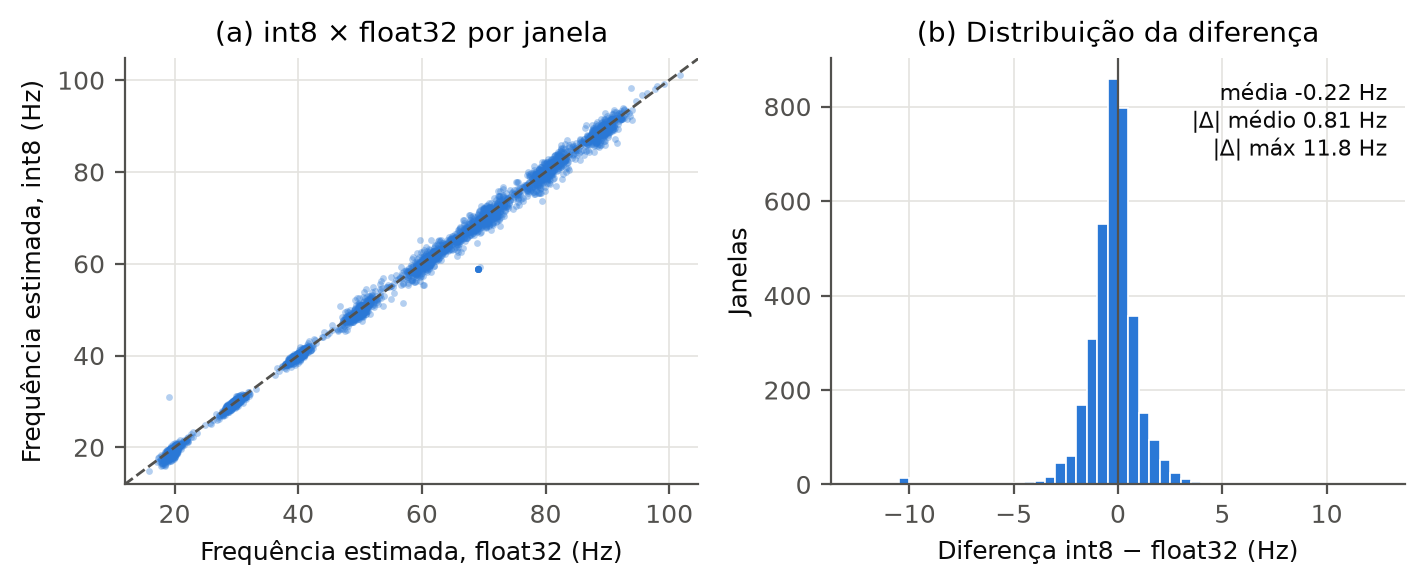
\includegraphics[width=\textwidth]{figs/embarcado/fig_quantizacao.png}
	\caption{Efeito da quantização int8 sobre a frequência estimada nas 3\,540 janelas: (a) estimativa int8 contra float32, com a reta identidade tracejada; (b) distribuição da diferença.}
	\label{sim:fig:quantizacao}
\end{figure}

\begin{table}[htbp]
	\centering
	\small
	\caption{Concordância entre implementações (3\,540 janelas). ``Nível'' é a frequência arredondada a 10\,Hz.}
	\label{sim:tab:fidelidade}
	\begin{tabular}{L{0.42\textwidth}ccc}
		\toprule
		\textbf{Comparação} & \textbf{Classe igual} & \textbf{Nível igual} & \textbf{\(|\Delta f|\) máx.} \\
		\midrule
		C float32 \(\times\) \texttt{scikit-learn} & 100\,\% & 100\,\% & \(2{,}5\times10^{-4}\)\,Hz \\
		C int8 \(\times\) emulação int8 (Python) & 100\,\% & 100\,\% & 0 (bit a bit) \\
		int8 \(\times\) float32 (efeito da quantização) & 98,2\,\% & 96,6\,\% & 11,8\,Hz \\
		Cadeia em C, percentis exatos \(\times\) Python int8 & 100\,\% & 100\,\% & 1,2\,Hz \\
		Cadeia em C, histograma \(\times\) Python int8 & 97,4\,\% & 96,2\,\% & 6,4\,Hz \\
		\bottomrule
	\end{tabular}
\end{table}

\subsubsection{Descritores e cadeia completa (V2)}

As fórmulas da Equação~\eqref{sim:eq:conversao}, aplicadas aos campos brutos, reproduziram as colunas físicas do \texttt{hits.csv} com erro relativo de no máximo \(10^{-5}\), compatível com o arredondamento do próprio arquivo. A Figura~\ref{sim:fig:descritores} mostra o erro normalizado máximo de cada descritor, nos dois canais, partindo do registro bruto. No modo exato, todos os erros ficaram abaixo de \(10^{-5}\), no nível da precisão simples; taxas e frações foram exatas, e os valores NaN coincidiram em todas as janelas. No modo histograma, os percentis ficaram acima da tolerância, como esperado de uma quantização em classes de largura fixa, com erros de até 0,2\,dB na amplitude, 0,04 nos logaritmos e 1,5\,kHz na frequência média.

\begin{figure}[htbp]
	\centering
	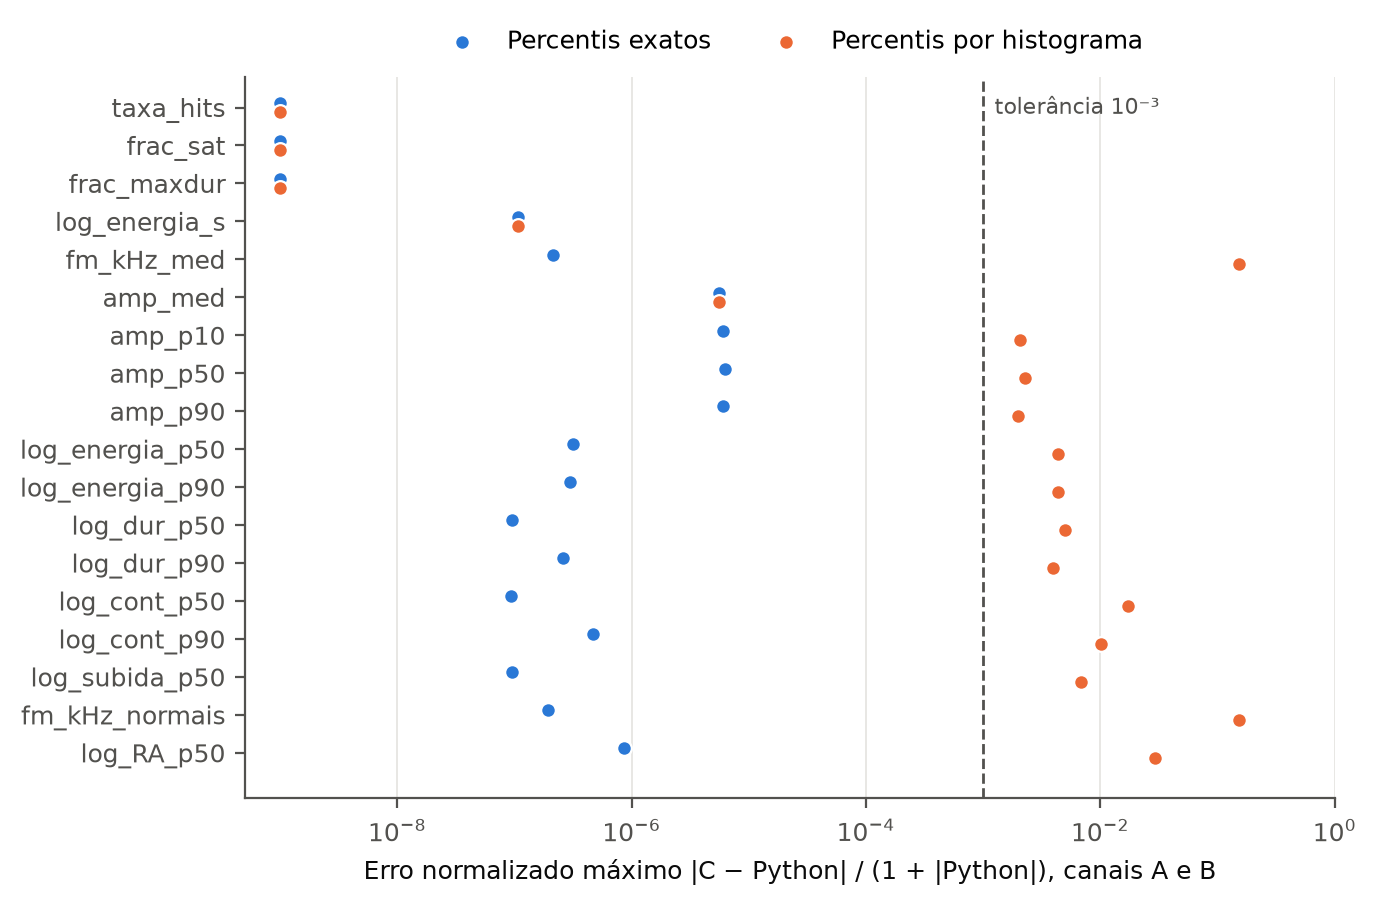
\includegraphics[width=0.92\textwidth]{figs/embarcado/fig_erro_descritores.png}
	\caption{Erro normalizado máximo, \(|x_{\mathrm{C}} - x_{\mathrm{Py}}|/(1+|x_{\mathrm{Py}}|)\), de cada descritor calculado em C a partir do registro bruto, nos dois modos de percentis, sobre as 3\,540 janelas e os dois canais. Erros nulos são desenhados em \(10^{-9}\). A linha tracejada é a tolerância de \(10^{-3}\).}
	\label{sim:fig:descritores}
\end{figure}

O que importa para a aplicação é a saída das redes. Com percentis exatos, a cadeia completa em C devolveu a mesma classe e o mesmo nível de frequência que o Python em 100\,\% das janelas; a maior diferença de frequência, 1,2\,Hz, vem do arredondamento da amplitude no \texttt{hits.csv}, que o C não usa ao partir do registro bruto. Com histogramas, a classe coincidiu em 97,4\,\% e o nível em 96,2\,\% (Tabela~\ref{sim:tab:fidelidade}), uma perda comparável à da própria quantização.

\subsubsection{Núcleo em lógica dedicada (V3 e V4)}

A simulação C e a cossimulação C/RTL do núcleo HLS, com 256 janelas, terminaram sem nenhuma divergência nos acumuladores ou na classe. A latência das duas redes foi de 11\,391 ciclos na síntese e de 11\,268 a 11\,393 ciclos na cossimulação, ou cerca de 114\,\(\mu\)s a 100\,MHz. Cada neurônio custa o número de entradas mais cerca de 12 ciclos de enchimento do \textit{pipeline}.

A Tabela~\ref{sim:tab:recursos} compara a estimativa da síntese HLS com o resultado após posicionamento e roteamento fora de contexto. A temporização foi atendida com folga: o caminho crítico tem 6,84\,ns, o que admitiria cerca de 146\,MHz. A implementação ocupou bem menos LUTs que a estimativa (656 contra 2\,421), porque a síntese lógica absorve parte da lógica de controle, e mais DSPs (14 contra 10), por causa da multiplicação de 64 bits da requantização. Os 3,5 blocos de BRAM guardam os 8\,960 pesos int8 das duas redes.

\begin{table}[htbp]
	\centering
	\small
	\caption{Recursos do IP HLS no XC7A35T (100\,MHz).}
	\label{sim:tab:recursos}
	\begin{tabular}{lrrrr}
		\toprule
		\textbf{Recurso} & \textbf{Estimativa HLS} & \textbf{Pós-roteamento} & \textbf{Disponível} & \textbf{Uso} \\
		\midrule
		LUT & 2\,421 & 656 & 20\,800 & 3,2\,\% \\
		\textit{Flip-flops} & 1\,648 & 682 & 41\,600 & 1,6\,\% \\
		DSP48E1 & 10 & 14 & 90 & 15,6\,\% \\
		BRAM (blocos de 36\,kb) & 3,5 & 3,5 & 50 & 7,0\,\% \\
		Período (ns) & 7,00 & 6,84 & 10,00 (alvo) & --- \\
		\bottomrule
	\end{tabular}
\end{table}

\subsubsection{Programa na MicroBlaze (V5)}

As seis simulações RTL (três programas \(\times\) duas configurações do processador) terminaram com a mesma sequência de valores de resultado da execução no computador: mesmas classes, mesmos acumuladores e, no modo exato, nenhum descritor fora da tolerância. Isso confirma, no nível do processador, que o binário embarcado reproduz o modelo. A Tabela~\ref{sim:tab:ciclos} resume os ciclos medidos.

\begin{table}[htbp]
	\centering
	\small
	\caption{Ciclos medidos na simulação RTL da MicroBlaze (100\,MHz, memória local, sem caches). Com FPU, médias sobre 2 vetores (MLP) e 2 janelas reais com 163 \textit{hits} (cadeia); sem FPU, 1 vetor e 1 janela com 81 \textit{hits}.}
	\label{sim:tab:ciclos}
	\begin{tabular}{lrr}
		\toprule
		\textbf{Etapa} & \textbf{Sem FPU} & \textbf{Com FPU} \\
		\midrule
		MLP float32, duas redes & \mbMlpFloatSoft & \mbMlpFloatFpu \\
		Quantização da entrada & \mbQuantSoft & \mbQuantFpu \\
		Núcleo int8, duas redes & \mbMlpIntSoft & \mbMlpIntFpu \\
		Inferência int8 completa (\(\mu\)s) & \mbMlpIntSoftUs & \mbMlpIntFpuUs \\
		\midrule
		Por \textit{hit}, modo exato & \mbHitSoft & \mbHitFpu \\
		Por \textit{hit}, modo histograma & \mbHitHistSoft & \mbHitHistFpu \\
		Fechar a janela, modo exato & \mbFecharSoft & \mbFecharFpu \\
		Fechar a janela, modo histograma & \mbFecharHistSoft & \mbFecharHistFpu \\
		\bottomrule
	\end{tabular}
\end{table}

\mbParagrafoMlp

A Figura~\ref{sim:fig:latencia} compara a latência da inferência nas plataformas. A Figura~\ref{sim:fig:ciclosjanela} decompõe o custo de uma janela típica dos dados (cerca de 80 \textit{hits}), e a Figura~\ref{sim:fig:carga} extrapola, a partir dos ciclos medidos, a ocupação da CPU em função da taxa de \textit{hits}.

\begin{figure}[htbp]
	\centering
	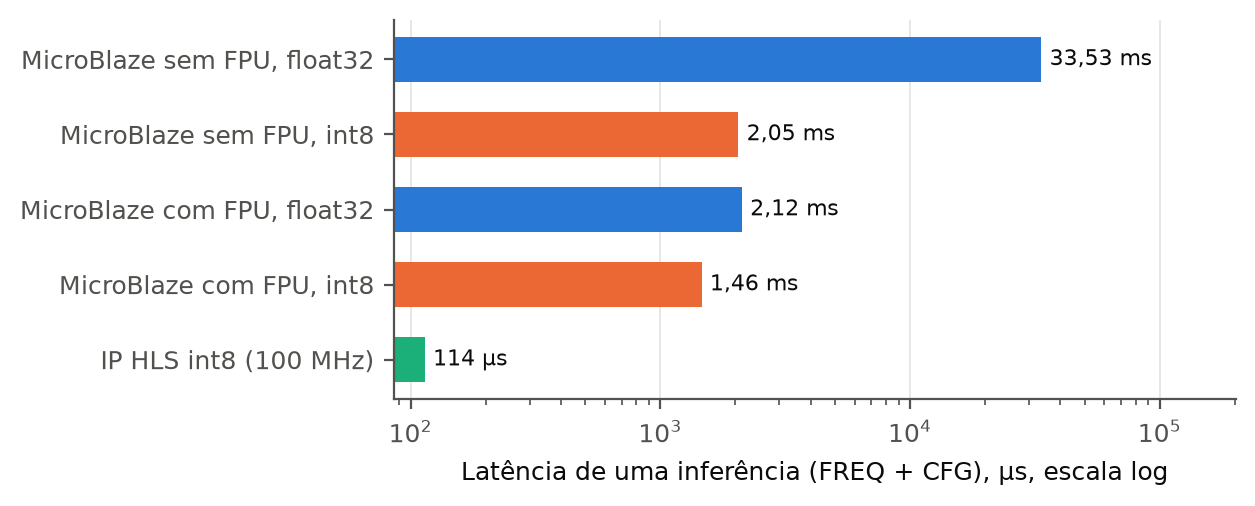
\includegraphics[width=0.85\textwidth]{figs/embarcado/fig_latencia_mlp.png}
	\caption{Latência de uma inferência (regressor e classificador) na MicroBlaze, medida em simulação RTL, e no IP HLS, medida na cossimulação. A MicroBlaze int8 inclui a quantização da entrada.}
	\label{sim:fig:latencia}
\end{figure}

\begin{figure}[htbp]
	\centering
	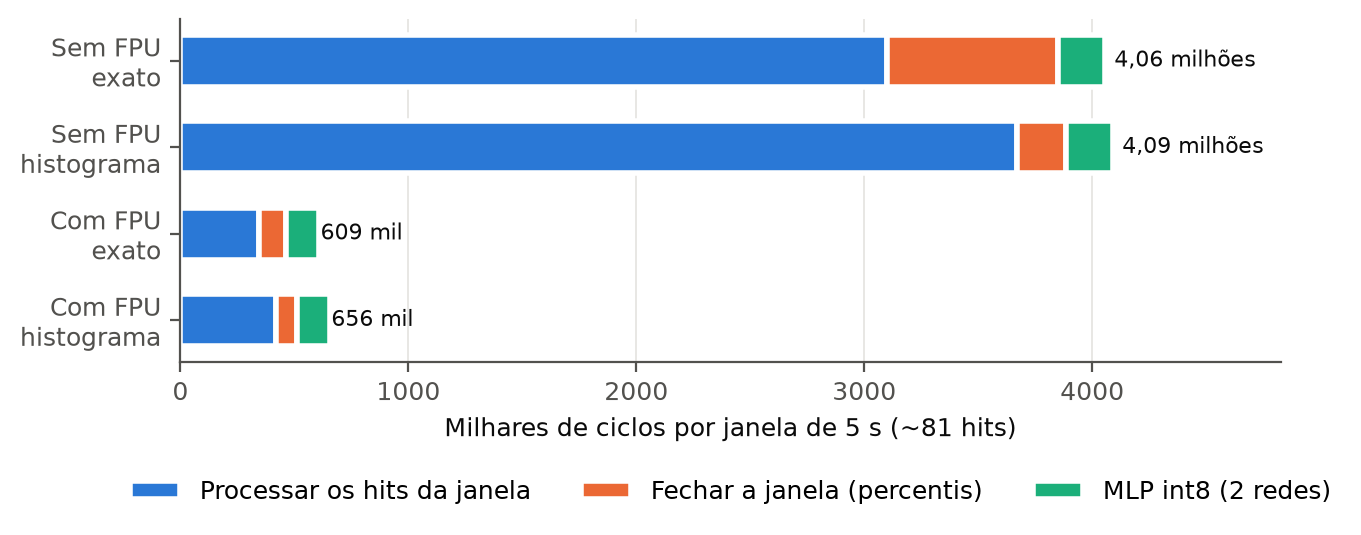
\includegraphics[width=0.92\textwidth]{figs/embarcado/fig_ciclos_janela.png}
	\caption{Composição dos ciclos de uma janela de 5\,s na MicroBlaze, para uma janela real de 81 \textit{hits} (custos por \textit{hit} medidos): processamento dos \textit{hits}, fechamento da janela (percentis) e MLP int8.}
	\label{sim:fig:ciclosjanela}
\end{figure}

\begin{figure}[htbp]
	\centering
	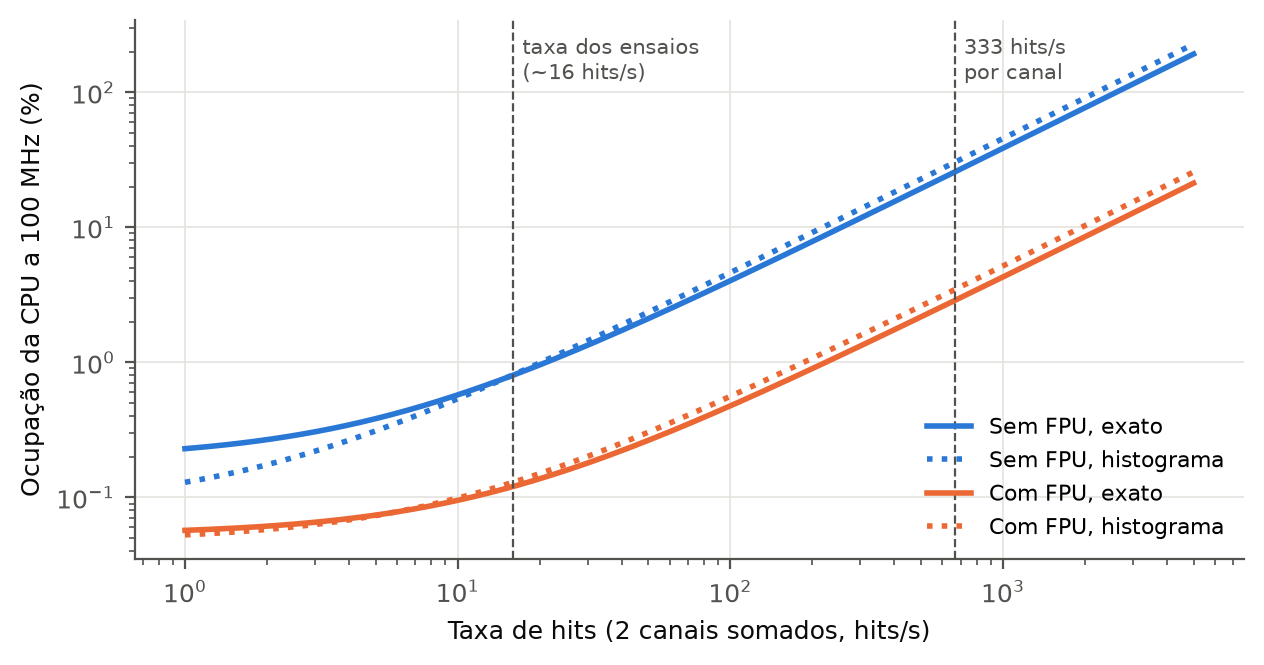
\includegraphics[width=0.85\textwidth]{figs/embarcado/fig_carga_cpu.png}
	\caption{Ocupação da CPU da MicroBlaze a 100\,MHz pela cadeia embarcada em função da taxa de \textit{hits}, extrapolada dos ciclos medidos por \textit{hit}, por fechamento de janela e pela MLP. As linhas verticais marcam a taxa dos ensaios da bomba e a maior taxa sustentada em ensaio elétrico. No modo exato, o fechamento da janela foi medido com cerca de 80 \textit{hits} e cresce como \(n \log n\); a extrapolação o subestima em taxas altas, e acima de 1\,024 \textit{hits} por canal por janela (cerca de 205 \textit{hits}/s por canal) o modo exato deixa de se aplicar.}
	\label{sim:fig:carga}
\end{figure}

\mbParagrafoCarga

A Tabela~\ref{sim:tab:memoria} resume a memória. O binário de teste da cadeia, com a MLP int8 e sem o caminho float32, ocupa de \mbTextoMin{} a \mbTextoMax\,kB de código e constantes, incluindo cerca de 10\,kB de \textit{hits} de teste que não existem no firmware real.

\begin{table}[htbp]
	\centering
	\small
	\caption{Memória da cadeia embarcada (ELF de teste, \texttt{mb-gcc} 2022.2, \texttt{-O2}).}
	\label{sim:tab:memoria}
	\begin{tabular}{lrr}
		\toprule
		\textbf{Item} & \textbf{Sem FPU} & \textbf{Com FPU} \\
		\midrule
		Código e constantes, modo exato (kB) & \mbTextoExatoSoft & \mbTextoExatoFpu \\
		Código e constantes, modo histograma (kB) & \mbTextoHistSoft & \mbTextoHistFpu \\
		Estado da janela, modo exato (kB) & 65,6 & 65,6 \\
		Estado da janela, modo histograma (kB) & 10,3 & 10,3 \\
		Pesos int8 e vieses das duas redes (kB) & \(\approx 9{,}8\) & \(\approx 9{,}8\) \\
		Pesos float32 das duas redes, se usados (kB) & \(\approx 37\) & \(\approx 37\) \\
		\bottomrule
	\end{tabular}
\end{table}

% =======================================================================================================
\subsection{Discussão}
\label{sim:sec:discussao}

\subsubsection{Qual rota usar}

A Tabela~\ref{sim:tab:rotas} reúne o custo em lógica de cada alternativa. Os números da MicroBlaze vêm da síntese do mesmo sistema usado na simulação e servem para dimensionar o acréscimo da FPU; o processador em si já existe no MOMEA e não é um custo da cadeia.

\begin{table}[htbp]
	\centering
	\small
	\caption{Recursos lógicos no XC7A35T: núcleo da MicroBlaze (síntese) e IP HLS (pós-roteamento).}
	\label{sim:tab:rotas}
	\begin{tabular}{lrrrr}
		\toprule
		\textbf{Bloco} & \textbf{LUT} & \textbf{FF} & \textbf{DSP} & \textbf{BRAM (36\,kb)} \\
		\midrule
		MicroBlaze sem FPU (núcleo) & 1\,361 & 857 & 4 & --- \\
		MicroBlaze com FPU estendida (núcleo) & 2\,322 & 1\,599 & 6 & --- \\
		Acréscimo da FPU & 961 & 742 & 2 & --- \\
		IP HLS int8 (duas redes) & 656 & 682 & 14 & 3,5 \\
		Memória local de 128\,kB (sistema simulado) & 17 & 16 & --- & 32 \\
		\bottomrule
	\end{tabular}
\end{table}

Para a aplicação atual, uma decisão a cada 5\,s, as duas rotas sobram. \mbParagrafoRota{} O IP HLS é \mbFatorHls{} vezes mais rápido que a MicroBlaze sem FPU e libera o processador, ao custo de 14 DSPs e 3,5 blocos de BRAM; ele se justificaria para classificar cada \textit{hit} em taxas altas, para modelos maiores ou se a MicroBlaze já estiver saturada pela pilha de rede. Em qualquer caso, a parte cara da cadeia não é a rede, mas o processamento por \textit{hit}, dominado pelos logaritmos; esse custo é o mesmo nas duas rotas, porque os descritores ficam no processador. Se a taxa de \textit{hits} crescer muito, o próximo passo natural é calcular na lógica as grandezas por \textit{hit} (incluindo os logaritmos, por tabela) e deixar à MicroBlaze apenas o fechamento da janela.

Entre os modos de percentis, o exato é preferível enquanto a janela couber na memória, porque preserva a decisão do modelo de referência em todas as janelas. O histograma troca cerca de 2,6\,\% de classes diferentes por memória constante e custo por \textit{hit} independente da taxa. Histogramas mais finos reduziriam essa diferença.

\subsubsection{O que a simulação garante}

A cadeia de verificação estabelece, com critérios explícitos, que: (i) a exportação do modelo e a implementação em C reproduzem o modelo de referência, bit a bit no caso int8; (ii) os descritores calculados em C a partir do registro bruto reproduzem os da Seção~\ref{sec:mm_bomba}; (iii) o RTL gerado pelo HLS é funcionalmente idêntico ao C e fecha a temporização na peça do MOMEA; e (iv) o binário compilado para a MicroBlaze produz os mesmos resultados em um processador simulado no nível RTL, com custo de tempo medido em ciclos.

A simulação não cobre, porém, o que depende da placa e do sistema completo:
\begin{itemize}
	\item a integração com o projeto atual do MOMEA, cuja ocupação de recursos não foi verificada; os recursos do IP foram obtidos fora de contexto, e o sistema MicroBlaze simulado não é o do MOMEA;
	\item o tempo de parede no firmware real, com caches ou memória externa, interrupções, recepção dos registros e pilha UDP concorrendo pelo processador;
	\item a base de tempo da janela: no treino, as janelas usaram a hora de chegada dos registros no computador; na placa, usarão o relógio local. Com o carimbo de tempo de \textit{hardware} ainda não implementado, pequenas diferenças na fronteira das janelas são esperadas;
	\item o comportamento elétrico do \textit{front-end} e do conversor, incluindo a saturação observada nos ensaios da bomba (Seção~\ref{sec:mm_bomba}).
\end{itemize}

\subsubsection{O modelo continua sendo o limite}

A implementação não muda a capacidade de generalização do modelo. Na Seção~\ref{sec:res_bomba}, a frequência generalizou para corridas não vistas (erro médio de 4 a 6\,Hz), mas a configuração das válvulas não (21 a 28\,\% de acurácia por corrida deixada de fora, para 14\,\% de acaso), e os dados têm limitações sérias: uma única corrida por condição, ordem fixa, limiar variável entre sessões e 70\,\% dos \textit{hits} saturados (Seção~\ref{sec:mm_bomba}). A contribuição deste trabalho é a infraestrutura: um fluxo que leva qualquer modelo do mesmo formato do Python ao FPGA, com verificação automática em cada nível. Retreinar com dados melhores exige apenas regenerar os cabeçalhos e repetir os testes; o código e o \textit{hardware} não mudam.

% =======================================================================================================


% -------------------------------------------------------------------------------------------------------
\section{Validação externa na base CWRU}
\label{sec:res_cwru}
% Gerado por ferramentas/importar_relatorios.py a partir de CWRU/RELATORIO_CWRU-10.11.2026/RELATORIO_CWRU.tex.
% Revisado à mão na dissertação: edite este arquivo, não a fonte.
\subsection{Resultados}
\label{cwru:sec:resultados}

\subsubsection{Os \textit{hits} capturam a física do defeito, mas só com limiar flutuante}

A Figura~\ref{cwru:fig:sinais} mostra trechos de 60\,ms das quatro condições, com os \textit{hits} detectados. Na pista externa, os impactos são nítidos e espaçados de cerca de 9\,ms, mas o anel de cada impacto permanece acima de 0,3\,\(g\) por vários milissegundos. Na pista interna, com RMS de 0,58\,\(g\), o sinal fica acima do limiar fixo quase o tempo todo. Com limiar fixo, os impactos se fundem: na gravação IR de 0,007~polegada com carga 0, 95\,\% dos \textit{hits} foram truncados pela duração máxima, e em três das quatro gravações IR de 0,021~polegada, cerca de 50\,\%. É o mesmo regime de emissão contínua observado nos ensaios da bomba. Com o limiar flutuante, a fração truncada caiu para no máximo 1\,\% em todas as gravações.

\begin{figure}[htbp]
	\centering
	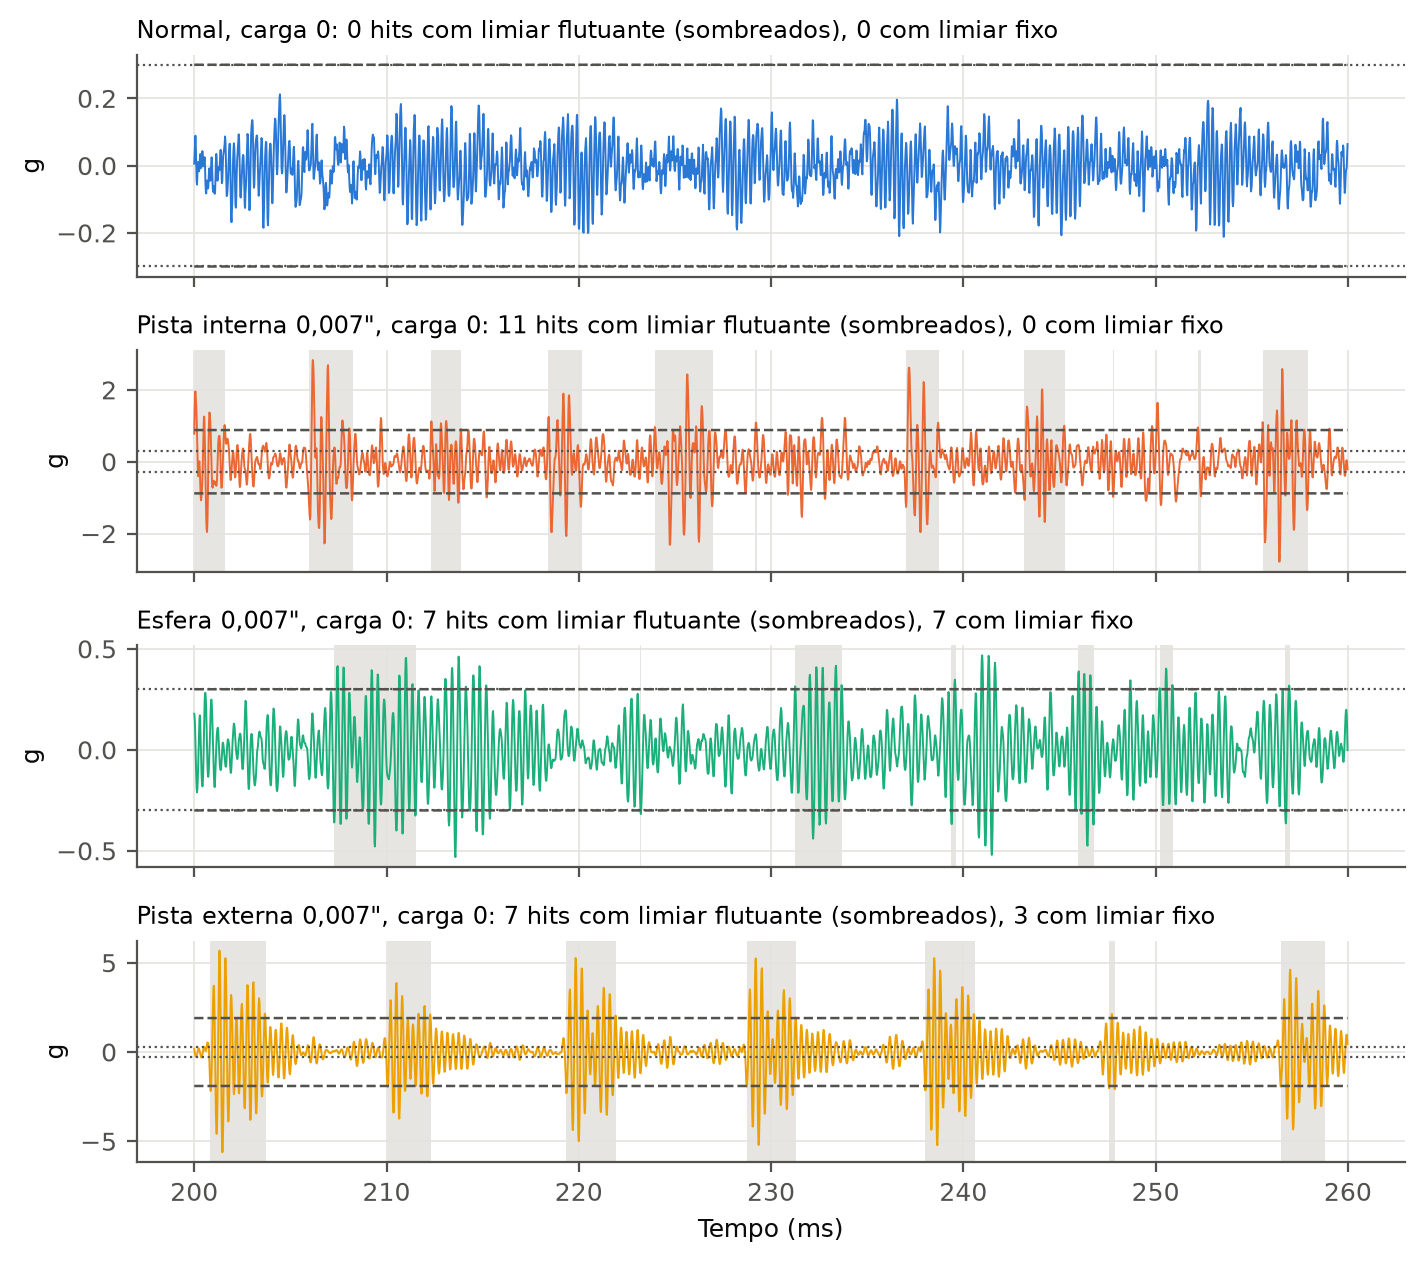
\includegraphics[width=\textwidth]{figs/cwru/fig_sinais_hits.png}
	\caption{Trechos de 60\,ms das quatro condições (carga 0, diâmetro de 0,007~polegada). Linhas pontilhadas: limiar fixo de 0,3\,\(g\); tracejadas: limiar flutuante. Áreas sombreadas: \textit{hits} detectados com o limiar flutuante.}
	\label{cwru:fig:sinais}
\end{figure}

A Figura~\ref{cwru:fig:ordem} mostra a ordem do intervalo entre \textit{hits}. Com limiar fixo, as distribuições são largas e têm picos espúrios perto de 1 e 2, que vêm de \textit{hits} fundidos e truncados. Com limiar flutuante, a pista externa concentra-se em 3,60 (BPFO = 3,58) e a pista interna em 5,27 (BPFI = 5,42); o pequeno desvio da pista interna é compatível com impactos perdidos quando o defeito sai da zona de carga. A esfera fica dispersa em torno de 5,5, longe de 2\(\times\)BSF = 4,71, o que concorda com a dificuldade conhecida de diagnosticar os defeitos de esfera dessa base \cite{smith2015}. Esse descritor é obtido sem FFT, apenas com os instantes dos \textit{hits}, o que reforça a importância do carimbo de tempo de \textit{hardware} ainda pendente no MOMEA.

\begin{figure}[htbp]
	\centering
	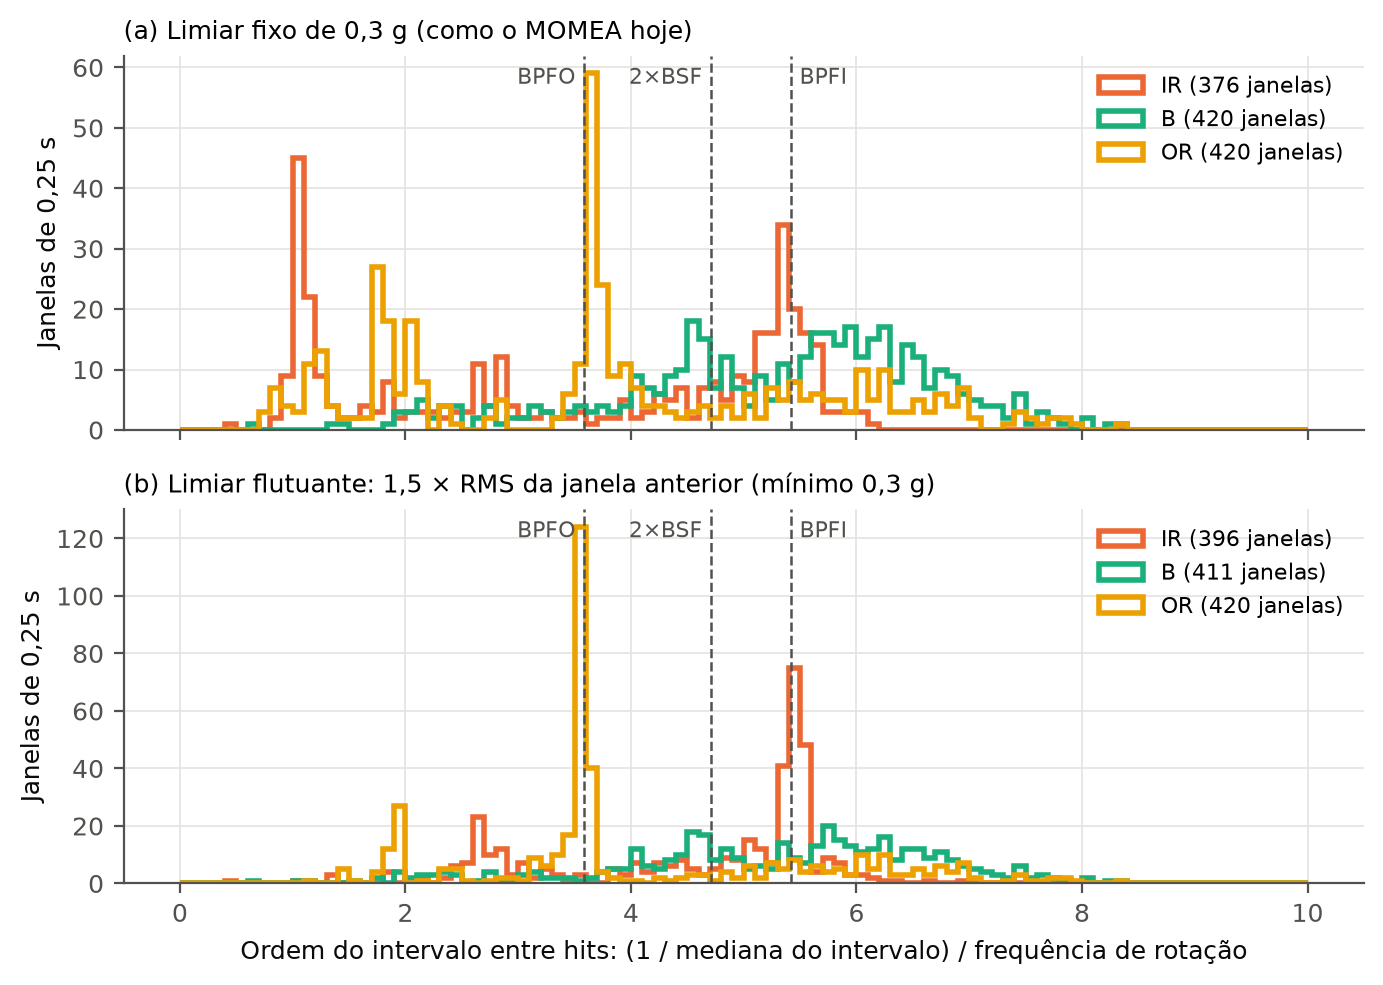
\includegraphics[width=\textwidth]{figs/cwru/fig_ordem_ihi.png}
	\caption{Ordem do intervalo entre \textit{hits} por janela, (a) com limiar fixo e (b) com limiar flutuante. Linhas tracejadas: frequências de defeito teóricas em múltiplos da rotação.}
	\label{cwru:fig:ordem}
\end{figure}

\subsubsection{A acurácia depende da validação}

A Figura~\ref{cwru:fig:acuracia} e a Tabela~\ref{cwru:tab:acuracia} resumem a classificação em quatro classes. Com janelas sorteadas, todos os grupos chegaram a 87--92\,\%, e as diferenças entre eles são pequenas. Deixar uma carga de fora quase não mudou o quadro (82--90\,\%), o que, à primeira vista, sugeriria boa generalização. Não é o caso: o teste ainda contém os mesmos rolamentos físicos, gravados em outra carga.

Quando o diâmetro inteiro sai do treino, a acurácia cai para perto do acaso nos descritores de amplitude: 21\,\% para os clássicos e 25\,\% para os \textit{hits} com limiar fixo, com a MLP. Os \textit{hits} com limiar flutuante sustentaram 46\,\% (53\,\% com RF), e o envelope, que mede diretamente as frequências de defeito, 63\,\%. Juntar todos os descritores não ajudou a MLP (41\,\%): os descritores de amplitude dominam o ajuste e não se transferem entre rolamentos, porque a severidade não é monotônica. Por exemplo, o defeito de 0,014~polegada na pista externa tem RMS de 4 a 8 vezes menor que os de 0,007 e 0,021. Na tarefa de dez classes, a queda das janelas sorteadas para a carga de fora foi um pouco maior (por exemplo, de 91 para 87\,\% com todos os descritores).

\begin{figure}[htbp]
	\centering
	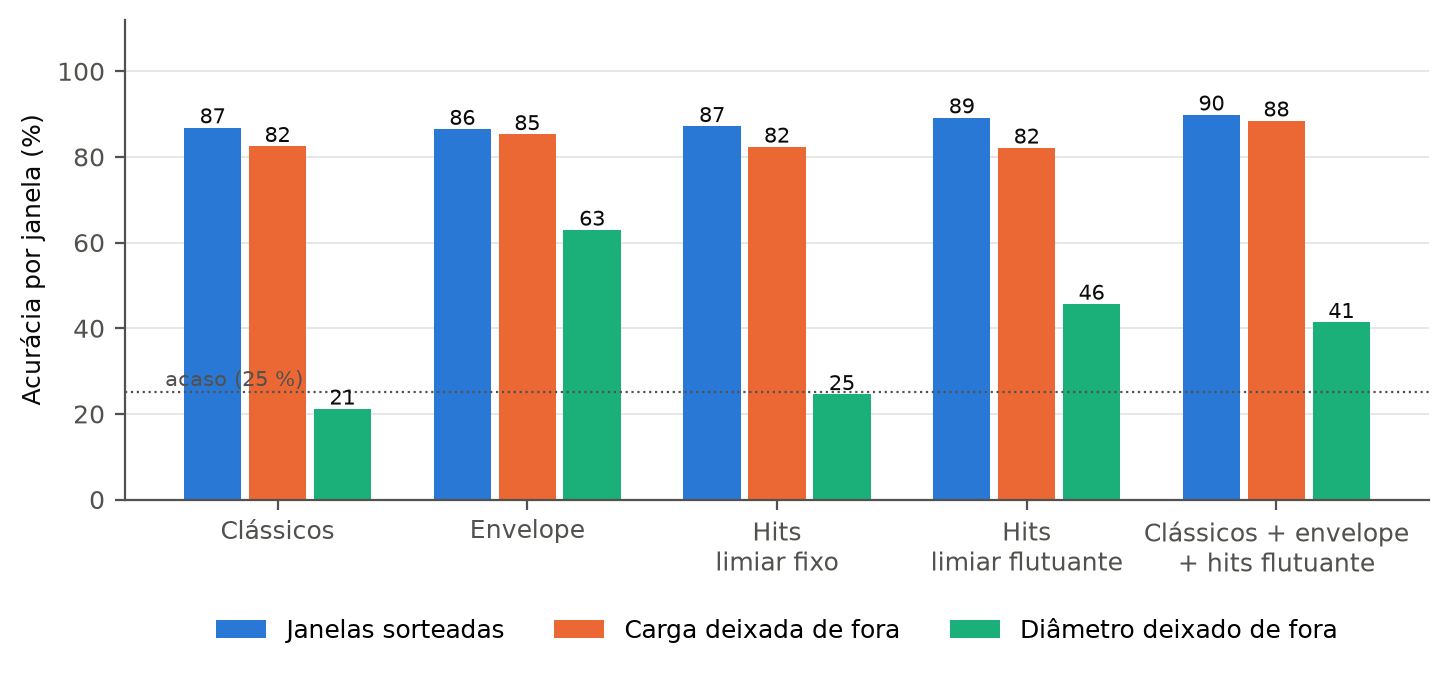
\includegraphics[width=\textwidth]{figs/cwru/fig_acuracia_validacoes.png}
	\caption{Acurácia por janela da MLP em quatro classes, por grupo de descritores e validação. A linha pontilhada marca o acaso (25\,\%).}
	\label{cwru:fig:acuracia}
\end{figure}

\begin{table}[htbp]
	\centering
	\small
	\caption{Acurácia por janela em quatro classes (entre parênteses, por gravação, com voto majoritário).}
	\label{cwru:tab:acuracia}
	\begin{tabular}{llccc}
		\toprule
		\textbf{Descritores} & \textbf{Modelo} & \textbf{Sorteada} & \textbf{Carga de fora} & \textbf{Diâmetro de fora} \\
		\midrule
		Clássicos & MLP & 86,8 (87,5) & 82,5 (82,5) & 21,2 (25,6) \\
		 & RF & 89,5 (92,5) & 86,4 (87,5) & 28,4 (28,2) \\
		Envelope & MLP & 86,5 (90,0) & 85,2 (90,0) & \textbf{62,9} (66,7) \\
		 & RF & 87,4 (90,0) & 85,8 (90,0) & 58,0 (59,0) \\
		\textit{Hits}, limiar fixo & MLP & 87,1 (90,0) & 82,3 (85,0) & 24,6 (20,5) \\
		 & RF & 88,7 (95,0) & 84,4 (80,0) & 35,3 (38,5) \\
		\textit{Hits}, limiar flutuante & MLP & 89,2 (92,5) & 82,1 (82,5) & 45,7 (43,6) \\
		 & RF & 90,5 (92,5) & 87,9 (90,0) & 53,3 (51,3) \\
		Todos (flutuante) & MLP & 89,8 (90,0) & 88,4 (87,5) & 41,4 (38,5) \\
		 & RF & 91,9 (90,0) & 89,6 (87,5) & 54,3 (51,3) \\
		\bottomrule
	\end{tabular}
\end{table}

A Figura~\ref{cwru:fig:confusao} mostra onde os erros se concentram, para os \textit{hits} com limiar flutuante. A máquina sã é sempre reconhecida, porque não gera \textit{hits}; o problema está em distinguir os defeitos entre si. Com o diâmetro de fora, a pista externa é confundida principalmente com a interna, e a esfera se divide entre as três classes de defeito.

\begin{figure}[htbp]
	\centering
	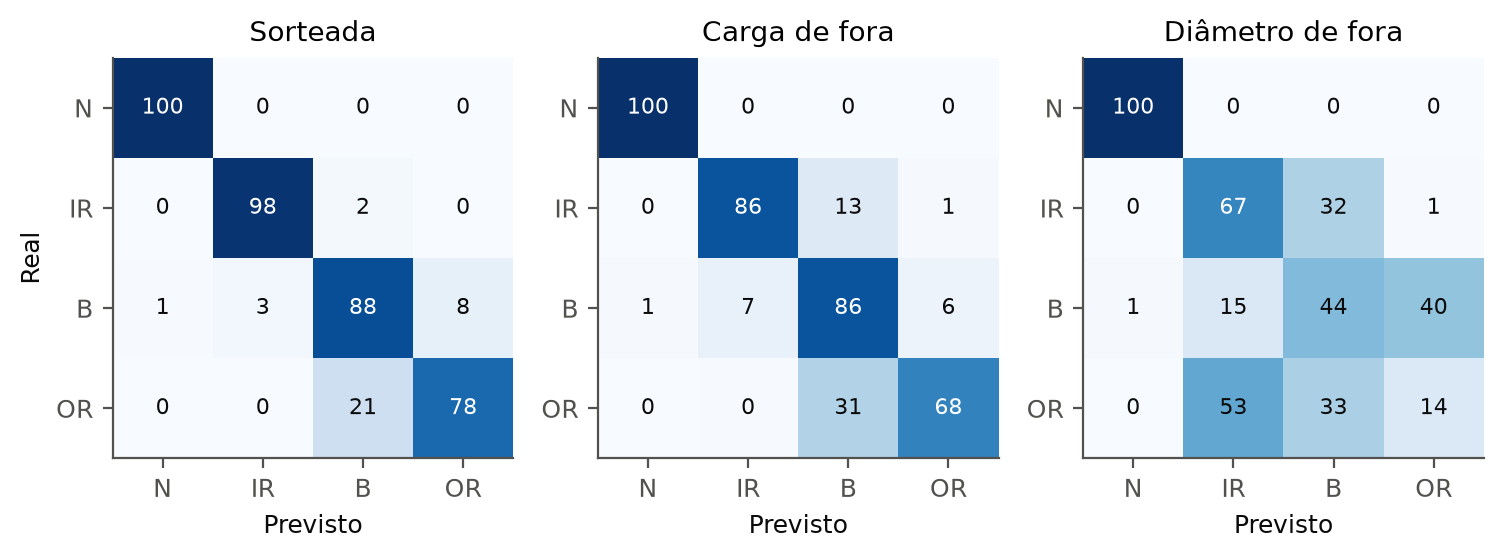
\includegraphics[width=\textwidth]{figs/cwru/fig_confusao_hits.png}
	\caption{Matrizes de confusão (\% por linha) da MLP com descritores de \textit{hits} e limiar flutuante, nas três validações.}
	\label{cwru:fig:confusao}
\end{figure}

\subsubsection{MLP int8}

Em cada parte da validação por carga, a MLP treinada foi quantizada para int8 com a mesma aritmética da implementação embarcada (Seção~\ref{sec:mm_embarcado}): escala de entrada fixa, pesos simétricos por camada e requantização inteira, com escalas calibradas apenas no treino da parte. A Tabela~\ref{cwru:tab:int8} mostra que a decisão int8 coincidiu com a de ponto flutuante em 98,4 a 100\,\% das janelas, e que a acurácia mudou no máximo 0,5 ponto percentual.

\begin{table}[htbp]
	\centering
	\small
	\caption{MLP em ponto flutuante e em int8 na validação por carga (quatro classes; faixas sobre as quatro partes).}
	\label{cwru:tab:int8}
	\setlength{\tabcolsep}{4pt}
	\begin{tabular}{lccccc}
		\toprule
		\textbf{Descritores} & \textbf{Entradas} & \textbf{MACs} & \textbf{Acc. float} & \textbf{Acc. int8} & \textbf{Concordância} \\
		\midrule
		\textit{Hits}, limiar flutuante & 14 & 3\,072 & 74,3--88,5\,\% & 73,8--88,2\,\% & 99,5--99,7\,\% \\
		Todos & 29 & 4\,032 & 86,5--90,5\,\% & 86,0--90,5\,\% & 98,4--100\,\% \\
		\bottomrule
	\end{tabular}
\end{table}

\subsubsection{Custo embarcado}

Os custos a seguir são estimativas derivadas dos ciclos medidos na simulação RTL da MicroBlaze a 100\,MHz (Seção~\ref{sec:mm_embarcado}), e não medições específicas para esta base:
\begin{itemize}
	\item \textbf{detecção dos \textit{hits}}: na lógica, como no MOMEA. A 48\,kHz, o detector é trivial para o FPGA;
	\item \textbf{descritores de \textit{hits}}: o custo medido foi de 4\,232 ciclos por \textit{hit} com FPU e 38\,287 sem. Na maior taxa observada (178 \textit{hits}/s), isso dá cerca de 0,8\,\% e 6,8\,\% da CPU, respectivamente;
	\item \textbf{MLP int8 com 14 entradas}: 3\,072 multiplicações-acumulações, ou cerca de 48 mil ciclos por janela (15,5 ciclos por operação, medidos), isto é, 0,5\,ms a cada 0,25\,s, ou 0,2\,\% da CPU;
	\item \textbf{envelope}: exige filtragem, transformada de Hilbert e FFT por janela. Com \(N = 16\,384\) pontos, cada FFT complexa custa cerca de \(5N\log_2 N \approx 1{,}1\) milhão de operações de ponto flutuante, e são necessárias pelo menos três. Isso dá da ordem de 3 a 4 milhões de operações por janela, ou 12 a 16 milhões por segundo. É inviável na MicroBlaze sem FPU e exigiria um núcleo de FFT na lógica.
\end{itemize}
Há, portanto, um compromisso claro: o envelope generaliza melhor entre rolamentos, mas custa uma FFT por janela; os \textit{hits} com limiar flutuante ficam a meio caminho, por uma fração do custo, e cabem na arquitetura atual do MOMEA.

% =======================================================================================================
\subsection{Discussão}
\label{cwru:sec:discussao}

\subsubsection{O que este estudo acrescenta à dissertação}

Os resultados reproduzem, numa base pública, as duas lições do estudo da bomba.
\begin{itemize}
	\item \textbf{A validação precisa separar as unidades físicas.} Janelas sorteadas e até cargas deixadas de fora deram 82--92\,\% com qualquer grupo de descritores, porque o modelo reconhece o rolamento, e não o tipo de defeito. Só separando os rolamentos a diferença entre os descritores aparece. É o mesmo padrão do LORO na bomba, em que a configuração das válvulas caiu de 89--95\,\% para 21--28\,\%. Na CWRU, porém, sabe-se que os defeitos são reais e localizados, de modo que a queda não pode ser atribuída à falta de efeito físico; ela vem da pouca diversidade de unidades (nove rolamentos com defeito e um são).
	\item \textbf{O limiar fixo do extrator falha diante de emissão contínua.} Com limiar fixo, os impactos se fundiram e foram truncados pela duração máxima, e os descritores de \textit{hits} ficaram no acaso fora da amostra. Com um limiar flutuante, os \textit{hits} recuperaram a periodicidade do defeito e a acurácia quase dobrou. Isso dá uma recomendação concreta para o MOMEA: oferecer um limiar flutuante na lógica, junto com a revisão do ganho já indicada pelos ensaios da bomba.
\end{itemize}

\subsubsection{Limitações}

\begin{itemize}
	\item Os sinais são de vibração, a 48\,kHz; nem os descritores nem as conclusões se transferem diretamente para EA de alta frequência ou para cavitação.
	\item O fator do limiar flutuante e o DDT foram escolhidos com base na concordância com as frequências de defeito, o que usa os rótulos; o ganho na validação por diâmetro pode estar ligeiramente otimista.
	\item Há apenas três partes na validação por diâmetro e nove rolamentos com defeito, de modo que as acurácias fora da amostra têm grande incerteza.
	\item Os defeitos são artificiais (eletroerosão) e únicos por condição; algumas gravações são atípicas, e os defeitos de esfera dessa base são sabidamente difíceis \cite{smith2015}.
	\item Os custos embarcados são estimativas a partir de medições em outra cadeia; o caminho completo para esta base não foi simulado em RTL.
\end{itemize}

% =======================================================================================================


% -------------------------------------------------------------------------------------------------------
\section{Discussão integrada}
\label{sec:discussao_integrada}

As seções anteriores avaliaram, separadamente, cada parte da cadeia. Esta seção as reúne em torno das perguntas que orientaram o trabalho, várias delas levantadas na qualificação.

\subsection{O que se ganha com a extração de \textit{hits} seguida de uma MLP?}

A extração de \textit{hits} resolve o problema de volume. Com registros de 32 bytes, o fluxo de um canal cai de 20\,MB/s para cerca de 26\,kB/s, incluindo os cabeçalhos de rede, na maior taxa ensaiada (redução global de cerca de 770 vezes; Seção~\ref{sec:res_extrator}). Isso dispensa a compactação contínua e a escrita de alta vazão que a plataforma USB exigia (Seção~\ref{sec:mm_antecedentes}) e permite transmitir por Ethernet a 100\,Mb/s. O extrator reproduziu as convenções temporais do sistema comercial e registrou de 99,94 a 99,96\,\% dos estímulos, sem perda na comunicação.

A extração, porém, não diz em que condição a máquina está. Um \textit{hit} é um evento; a condição aparece na estatística dos eventos ao longo do tempo. Por isso a classificação usa descritores por janela (taxa, percentis de amplitude, energia, duração, contagens e periodicidade), e não um limiar fixo sobre um único \textit{hit}. Nos ensaios da bomba, esses descritores permitiram estimar a frequência de rotação com erro médio de 4 a 6\,Hz em corridas não vistas (Seção~\ref{sec:res_bomba}). Na base CWRU, a ordem do intervalo entre \textit{hits} reproduziu as frequências teóricas de defeito dos rolamentos (Seção~\ref{sec:res_cwru}). Nenhum desses resultados seria obtido comparando cada \textit{hit} com um limiar.

\subsection{O sistema opera em tempo real?}

Depende da etapa. O extrator opera em tempo real: cada \textit{hit} é detectado e parametrizado na lógica, e o registro é emitido \(T_{\mathrm{DDT}} + T_{\mathrm{HLT}} = 2{,}25\,\mathrm{ms}\) após o último cruzamento, mais o serviço do DMA, do \textit{firmware} e da rede. Na plataforma USB, os dados passavam por um banco intermediário e eram analisados depois; com o extrator, os registros chegam à aplicação à medida que os eventos ocorrem.

A classificação, por construção, decide uma vez por janela. Com janelas de 5\,s, o atraso de decisão é de até 5\,s, mais o tempo de inferência, que é desprezível: de 1,5 a 2,1\,ms na MicroBlaze e 114\,\(\mu\)s no IP HLS (Seção~\ref{sec:res_embarcado}). Para o monitoramento de cavitação e de desgaste, cuja evolução ocorre em minutos ou horas, esse atraso é adequado. A janela é um compromisso entre estabilidade e rapidez: no estudo da bomba, janelas de 2\,s melhoraram ligeiramente o reconhecimento da frequência, mas aumentam a variância dos descritores quando a taxa de \textit{hits} é baixa.

\subsection{Quanto tempo de coleta é necessário para identificar uma condição?}

A resposta depende da taxa de \textit{hits}, porque os descritores são estatísticas da população de eventos. Nos ensaios da bomba, havia cerca de 30 a 50 \textit{hits} por canal em cada janela de 5\,s. Na base CWRU, com 60 a 180 impactos por segundo, janelas de 0,25\,s bastaram para estimar a periodicidade do defeito. Como regra prática, a janela precisa conter algumas dezenas de \textit{hits} e vários períodos do fenômeno de interesse. Em termos de coleta para \emph{treinar} o modelo, o fator limitante não foi a duração das gravações, mas o número de corridas independentes: com uma única corrida por condição, o modelo aprende a assinatura da corrida, e não a condição (Seções~\ref{sec:res_bomba} e~\ref{sec:res_cwru}).

\subsection{O FPGA tem capacidade para a cadeia completa?}

Para o fluxo de dados, sim: o detector processa as amostras a 10\,MSa/s na lógica, e a carga restante é proporcional à taxa de \textit{hits}, não à taxa de amostragem. Na MicroBlaze, a cadeia de descritores e a MLP ocupam menos de 1\,\% da CPU na taxa dos ensaios e cerca de 26\,\% sem FPU a 333 \textit{hits}/s por canal (Seção~\ref{sec:res_embarcado}).

Em recursos lógicos, a margem é pequena. Após a migração da FIFO para BRAM, o extrator de dois canais ocupa cerca de 92\,\% das LUTs do XC7A35T (Seção~\ref{sec:mm_implementacao}). O IP HLS da MLP acrescentaria 656 LUTs (3,2\,\%) e 14 DSPs, e a FPU da MicroBlaze, 961 LUTs (4,6\,\%). Ambas as opções caberiam, mas no limite, com risco para o fechamento temporal. A rota recomendada para o hardware atual é, portanto, a inferência int8 em software, na MicroBlaze já existente e sem FPU: ela não consome lógica adicional e cabe com folga no tempo disponível. O IP HLS e a FPU tornam-se justificáveis em um FPGA maior ou se a taxa de \textit{hits} crescer muito.

\subsection{Por que uma MLP, e não uma rede convolucional?}

Porque a entrada do classificador é um vetor de descritores, e não uma série temporal. A arquitetura proposta não transmite as amostras: o FPGA entrega registros de \textit{hits}, dos quais se calculam 36 descritores por janela. Uma rede convolucional unidimensional (CNN-1D) ou temporal exigiria a forma de onda, isto é, justamente o fluxo que se quer evitar. As redes convolucionais bidimensionais sobre espectrogramas, estudadas anteriormente no projeto, são compatíveis com a aquisição contínua, mas não com o processamento na borda proposto. A MLP é o modelo natural para um vetor curto de atributos, tem custo previsível (cerca de 4,6 mil multiplicações-acumulações por rede) e é simples de quantizar e de mapear em \textit{hardware}. Uma extensão possível é capturar seletivamente a forma de onda de alguns \textit{hits} e combiná-la com os descritores, o que é discutido como trabalho futuro.

\subsection{Como a MLP foi implementada no FPGA?}

Em vez de \textit{frameworks} como FINN ou hls4ml \cite{Umuroglu2017FINN,duarte2018}, que partem de modelos treinados em \textit{frameworks} de aprendizado profundo e visam redes maiores, optou-se por um núcleo próprio em C. O modelo do \texttt{scikit-learn} é exportado como tabelas de pesos int8, e um único código-fonte compila para a MicroBlaze e para o Vitis HLS. Isso manteve a aritmética sob controle a ponto de exigir igualdade bit a bit entre o Python, o C e o RTL gerado, o que um fluxo automatizado não garantiria com a mesma transparência.

\subsection{O que foi comparado e o que não foi}

A qualificação previa comparar a solução em FPGA com CPU e GPU quanto a eficiência, tempo de resposta e consumo. A comparação realizada foi entre as rotas viáveis no próprio FPGA (MicroBlaze sem e com FPU e acelerador HLS), com o computador como referência de exatidão. Comparar com uma GPU não faz sentido para duas redes de cerca de 4,6 mil operações cada, executadas uma vez a cada 5\,s: o custo é dominado pela transferência e pela inicialização, e não pelo cálculo. O consumo de energia não foi medido, porque exige a placa; as estimativas de potência das ferramentas de síntese não foram usadas como substitutas.

\subsection{Limites do que foi demonstrado}

Os resultados demonstram que o extrator é equivalente ao sistema comercial na faixa ensaiada, que os descritores de \textit{hits} contêm informação sobre a condição de operação e que a classificação pode ser executada no FPGA com fidelidade ao modelo de referência. Eles não demonstram que o sistema detecta cavitação em uma turbina. Os ensaios do extrator são elétricos, sem sensor nem propagação estrutural; o estudo da bomba tem uma única corrida por condição, saturação de 70\,\% dos \textit{hits} e limiar variável entre sessões; e a base CWRU é de vibração, com defeitos artificiais. Esses limites orientam os trabalhos futuros do Capítulo~\ref{chap:conclusoes}.
